\documentclass[a4paper, 12pt]{report}
%================================================================
\usepackage{verbatim, fancyhdr, theorem, dsfont, color,
            amsmath, amsfonts, amssymb,
            hyperref,epsfig, graphicx, setspace}
\usepackage{graphics}
\usepackage[margins]{trackchanges}
% to insert pdf sous la forme
% \includepdf[pages=-]{../CoherePart_CR1nov2012/rapportCoherence.pdf}
%\usepackage{pdfpages}
%============================================
 \textheight 23cm
% \doublespace
%  \oddsidemargin -0.5cm
% \evensidemargin +1.5cm
%  \textwidth 17cm
% \topmargin 0cm
%============================================
% Figures
%============================================
\newcommand{\figsstit}[2]{
\begin{figure}[hbtp]
\centerline{
    \hbox{ \epsfig{figure={#1}, scale=#2} }
}
\end{figure}}
%============================================
\newcommand{\figscale}[4]{
\begin{figure}[hbtp]
\centerline{
    \hbox{ \includegraphics[scale=#4]{#1} }
}
\begin{center}
\parbox{12	 cm}
{
    \caption{\protect\small\it  {#2}}
    \label {#3}
}
\end{center}

\end{figure}}

%%============================================
%\newcommand{\figsstit}[2]{
%\begin{figure}[hbtp]
%\centerline{
%    \hbox{ \includegraphics{figure={#1}, scale=#2} }
%}
%\end{figure}}
%

%==============================================
\newcommand{\prob}[1]{\mathds{P}\left( #1 \right)}
\newcommand{\esp}[1]{\mathds{E}\left[ #1 \right]}
\newcommand{\var}[1]{\mathrm{var}\left( #1 \right)}
\newcommand{\cov}[1]{\mathrm{cov}\left( #1 \right)}
\newcommand{\diag}[1]{\mathrm{diag}\left( #1 \right)}
\newcommand{\trace}[1]{\mathrm{trace}\left( #1 \right)}
\newcommand{\card}[1]{\left| #1 \right|}
\newcommand{\myemph}[1]{\emph{\color{red}#1}}


 \newcommand{\benoit}[1]{\marginpar{\color{red}\footnotesize{BENOIT:}
                \color{red}\footnotesize{ #1}}}

 \newcommand{\momo}[1]{\marginpar{\color{blue}\footnotesize{MOMO:}
                \color{blue}\footnotesize{ #1}}}
%%============================================================================
%\def\thesection{\arabic{section}.}
%\def\thesubsection{\arabic{section}.\arabic{subsection}}
%\def\thesubsubsection{\arabic{section}.\arabic{subsection}.\arabic{subsubsection}}
%\def\thefigure{\arabic{figure}}
%\def\theequation{\arabic{equation}}
%\def\theexercice{\arabic{exercice}}
%\def\theexample{\arabic{example}}
%\def\theproof{\arabic{proof}}

%===============================================
\newtheorem{property}{Properties}
\newtheorem{remark}{Remark}
\newtheorem{theorem}{Theorem - \thetheoreme}
\newtheorem{definition}{Definition - \thedefinision}
\newtheorem{example}{Example}
\newtheorem{lemme}{Lemme - \thelemme}
\newtheorem{proof}{Proof - \theproof}
\newenvironment{TAB}{\begin{table}[[hbt] \center \leavevmode}{\end{table}}
%%=========== LOGO/Head/Foot par PAGE ========
%\pagestyle{fancy}
% \lhead[]{}
% \chead[]{}
% \rhead[]{\includegraphics[scale=0.1]{\DIRLOGO/logo_telecomparis}}
% \lfoot[]{\thechapter}
% \cfoot[]{}
% \rfoot[]{\thepage}

%%============================================================================
%\newcounter{auxiliaire}
%%%%%%%% comment
%\setcounter{auxiliaire}{\theenumi}
%\end{enumerate}
% TEXTE
%\begin{enumerate}
%\setcounter{enumi}{\theauxiliaire}
%%============================================================================
%\renewcommand\arraystretch{1.6}

\def\ua{\underline a}
\def\ub{\underline b}
\def\uB{\underline B}
\def\uH{\underline H}
\def\ur{\underline r}
\def\us{\underline s}
\def\ux{\underline x}
\def\uX{\underline X}
\def\uZ{\underline Z}
\def\utheta{\underline \theta}
\def\hat{\widehat}

\def\MSC{\mathrm{MSC}}
\def\SNR{\mathrm{SNR}}
\def\iSNR{\mathrm{SNR}^{-1}}

\def\degree{$^{\circ}$}

\def\ut{{u}}
\def\rf{{r}}

%============== colors ========================
\definecolor{enstrouge}{RGB}{212,65,84}
\definecolor{lightorange}{RGB}{235,226,52}
\definecolor{greennoise}{RGB}{243,42,255}
\definecolor{lightred}{RGB}{255,181,183}
\definecolor{light-grey}{rgb}{0.95,0.95,0.95}
\definecolor{peach}{rgb}{0.98,0.49,0.25}
\definecolor{burntorange}{rgb}{0.79,0.37,0}
\definecolor{light-yellow}{rgb}{1,1,0.92}

\definecolor{light-green}{RGB}{231,255,145}
\definecolor{enstorange}{RGB}{255,214,10}
\definecolor{enstrouge}{RGB}{212,65,84}
\definecolor{grey}{RGB}{204,204,204}
\definecolor{blue}{RGB}{0,0,255}
\definecolor{almost-black}{RGB}{100,100,100}
\definecolor{violet}{rgb}{0.4,0,0.4}
\definecolor{cyan}{RGB}{0,255,255}
\definecolor{magenta}{RGB}{243,42,255}

\def\degree{^{\circ}}
\def\simiid{\stackrel{\mathrm{i.i.d.}}{\sim}}
\def\MSC{\mathrm{MSC}}%{\MSC}}
\def\hMSC{\widehat{\MSC}}%{\MSC}}


 \def\programsfullprocess{fullprocess/}
 \def\programsToolbox{fullprocess/ZZtoolbox/}
 \def\programspierrick{fullprocess/ZZtoolbox/00Pierrick/}



\graphicspath{{figures/}}
%============================================
\begin{document}
 \sloppy
%  \nocite{*}
 \bibliographystyle{plain}
\tableofcontents
%===========================================
%===========================================
%===========================================
%===========================================
\part{Theoretical aspects}
%===========================================
%===========================================
\chapter{Problem position}
% !TEX root = ../calibreport.tex
%===========================================
%===========================================
\section{Objective}
%===========================================


This study is devoted to the calibration of an infrasound system, which consists of its sensor and its Wind Noise Reduction System and which is assumed to be a linear time-invariant system, commonly called a linear filter in the literature.  It is expected that most results could be applied to the calibration of seismometers, using a reference instrument.\\*

The specifications set out in the Operational Manual \footnote{CTBT/WGB/TL-11,17/17/REV.5 Operational Manual for Infrasound Monitoring and the International Exchange of Infrasound Data} provide Minimum Requirements for the calibration of Infrasound Stations: the frequency response shall be within $\pm 5\%$ in amplitude gain from the nominal response in the PTS passband ($0.02$ Hz to $4$ Hz). That represents a challenging issue. 
It should be noted that no Minimum Requirements are listed for the phase response of Infrasound Stations, yet it is stated in part 4.5 Calibration of the Operational Manual, that: "The calibration minimum requirements for infrasound stations do not currently include phase measurement; however, these measurements are necessary to establish the full system response that is required for data processing at the International Data Centre."\\*


%================ figure ====================
\figscale{schema-of-observation-simple.pdf}{Measurement process. SUT denotes the sensor under test, it consists of a sensor and its noise reduction system. SREF denotes the reference sensor. SUT and SREF are assumed to be linear filters. $e_{u}(t)$ and $e_{u}(t)$ denote the non observable input signals. $x_{u}(t)$ and $x_{r}(t)$ are sampled and recorded.}{fig:schema-of-observation-simple}{0.8}


The method to estimate the response of a infrasound system, denoted System Under Test (SUT) in the following, is based on the use of a second sensor, denoted System of Reference (SREF), whose frequency response is perfectly known. The calibration method is based on the presence of a quasi permanent background signal all over the Word \cite{?}.  Still in \cite{?}, experimental results have shown that this background signal has a large enough frequency bandwidth and energy to satisfy the PTS requirements. \\*


This  background signal  induces two  signals denoted $e_{u}(t)$ and $e_{r}(t)$ in the figure \ref{fig:schema-of-observation-simple}
A useful property is that a large part of these two signals is simultaneously present  on the two sensors. The main reason of the presence of this same signal is related to the spatial coherence which is due to the fact that the signal wavelength is much larger than the distances  involved in the measurement process: for a common acoustical velocity of $300$ m/s, and the highest frequency of interest saying $4$ Hz, the wavelength is $75$ m which is much larger than the distance between the two sensors, which is less than 3 meters. 
\change[momo]{}{It is worth to notice that the air turbulences, which can be at first order characterized by the ratio $v/f$ where $v$ is its velocity of around a few meters per second, e.g. $4$ m/s, induces spatial coherence phenomena for frequencies under $f<0.02$ Hz, see chapter ...}

\change[momo]{}{In the following the common part, denoted $s(t)$, is shortly called the \emph{coherent signal}. However spatial coherence does not mean that there is a commun part for the inputs of the two sensors. It means that a part of the SUT signal is a filtering of a part of the SREF signal. But if such situation occurs, the filter involved is not identifiable. In the following we assume that this filter is the identity filter.  More specifically we let:}
\begin{eqnarray}
\label{eq:model-signal-introduction}
\left\{
\renewcommand\arraystretch{1.6}
\begin{array}{rcl}
e_{\ut}(t)&=&s(t)+w_{\ut}(t)
\\
e_{\rf}(t)&=&s(t)+w_{\rf}(t)
\end{array}
\right.
\end{eqnarray}
where $w_{\ut}(t)$ and $w_{\rf}(t)$ are such that the correlation between them are zero for any couple of times. In the following they are shortly called \emph{noise}.  They are mainly due to the wind.\\*

Unfortunately the signal $s(t)$ is not  \emph{observable}. It follows that, in presence of the additive noises $w_{\ut}(t)$ and $w_{\rf}(t)$, the problem is ill-conditioned in the sense that they are an infinity of possible solutions.






%Although the wind structure is very different of the  "acoustical'' signal $s(t)$, we will see that a parameter of interest is $\zeta=v/f$ where $v$ is the wind velocity and $f$ the frequency. $\zeta$ can be interpreted as a wavelength. \annote[Benoit]{For typical values of the wind velocity, $\zeta$ is much lower than the distances between air inlets of the noise reduction system (NRS).}{Je ne comprends pas bien l'int\'er\^et de cette phrase, surtout qu'a mon sens, en basse frequence le ratio $\zeta$ est presque toujours plus grand que la distance inter-inlet. Un aspect du probl\`eme consiste justement \`a comprendre et mod\'eliser le "dip" comme une fonction de $\zeta$, non ?}

%===========================================
 \newpage\clearpage
%===========================================
\section{Experimental testbed}
%===========================================
In may 2015, an experimental setup has been deployed in the IS26 located in Freyung in Germany:
\begin{itemize}
\item
The different sensors under test/reference are reported table \ref{tab:sensor-specifications}. Each reference sensor was installed in the same vault as the sensor under test, and was connected to a newly installed reference inlet through a short pipe. The reference inlet port was positioned at a short distance (less than a few meters) from the main manifold of the Wind Noise Reduction System. 
These sensors have been checked before installation. We have two kinds of SREF, one is MB2005, the other MB3. The SUT sensor is a MB3. For our calibration problem both SREF sensors can be considered as almost identical.
\item
The environment is particularly  quiet, due to the Bavarian Forest where the station is located. It follows that the wind is very low during large periods of time.

 \item
The data are recorded in continuous at the IDC, in testbed.
\end{itemize}

It is worth to notice that the calibration problem is a little bit different of the detection problem which consists to provide an alert when the system is out of specifications.


\begin{table}[h]
\begin{center}
\begin{tabular}{|c||cc|cc||}
\hline
Site & SUT & info.& SREF & info.
\\
\hline
     & model&serie \#     & model&serie \#
\\
H1/C1& MB3 & 00020  & MB2005& 6046
\\
H2/C2& MB3  &  00017  & MB2005& 5125
\\
H3/C3& MB3  &  00014  & MB2005 &6039
\\
H4/C4& MB3  &  00023  & MB2005& 5104
\\
H5/C5& MB3   & 00012  & MB2005 &7095
\\
H6/C6& MB3  &  00011  & MB3 &00007
\\
H7/C7& MB3   & 00021  & MB3 &00008
\\
H8/C8& MB3   & 00015  & MB3 &00022
\\
\hline
\end{tabular}
\parbox{12 cm}
{
    \caption{\protect\small\it  sensor specifications: all sensors have the same theoretical sensitivity of $0.02$ V/Pa. The MB3s have self noise lower than that of the MB2005s. The sites associated to the ''Wind Noise Reduction System" are labelled H whereas  the sites of reference sensors are labelled C. In the site 1, we have wind informations, as direction, velocity, etc}
    \label{tab:sensor-specifications}
}
\end{center}
\end{table}

%\figscale{H1-H5MB2005.jpg}{}{}{fig:H1-H5MB2005}

 \newpage
%===========================================
%===========================================
\section{Main issue}
%===========================================

The main issue is related to the under-determination of the problem (also known as blind identification). More specifically in our model we have four unknowns for only two observations. The four unknowns are the frequency response of the SUT, the spectral shape of the coherent signal and the spectral shapes of the two noises. The two observations are the output signals on both sensors, see figure \ref{fig:general-schema}.

A common way to solve this kind of problem is to introduce some {\it a priori} knowledges/assumptions. The drawback is what happens when the {\it a priori} knowledges are not well-verified.

Here a list of {\it a priori} knowledges that could be considered:
\begin{itemize}
\item
 the signals are stationary in the whole frequency bandwidth of interest. More specifically we have to precise what we mean in terms of stationarity duration. The worst case  is for the low frequency, i.e. for long period. For example if the target accuracy requires to integrate the signal over five periods and if we want to analyze the spectral content around the frequency of $0.01$ Hz, about $10$ minutes of stationarity are needed.
 
Let us notice that, even under the stationarity assumption the problem is still under-determined.
 

  \item
the coherent signal and the noises can be modeled with parametrical models such as auto-regressive paradigm. In \cite{frazier:2013} a generalized autoregressive conditionally heteroskedastic (GARCH) model has been used to model the wind. This approach has not been investigated here.

  \item
 the noises on the two sensors are uncorrelated and white. This is the simplest parametrical model which depends on only one parameter. In this case the frequency response is identifiable, but observations and also the physical aspects of the wind noises deny this assumption.
   \item
the system under test is a linear filter with {\it given} numbers of poles and zeroes (parametrical approach). This approach has not been already investigated. It follows that, for the calibration, implying the numbers of poles and zeroes could hide a singularity and then induce a bias. To illustrate this statement, saying that a system is of order 1 can hide in the estimated response the presence of a non suspected resonance. \annote[Benoit]{But in the alert issue framework, we  see that something is wrong, therefore we suspect that it could be an efficient way for test.}{A reformuler / preciser.} 

\item
assuming that the two noises are uncorrelated, the indetermination disappears if  we assume that the ratio between the two noise levels is known. That is a realistic way in high frequency because the NRS works well and the ratio is about the inverse of the number of inlets.

\item
assuming that the two noises are uncorrelated, the indetermination disappears if  we assume that one of the two noises is negligible, typically it could be the case for the SUT which is provided with a noise reduction system (NRS). But we also want to detect if this NRS is working well.

The advantage of the  assumption is that the second noise could be very large, we only have to use the formula \eqref{eq:ratio-sup}. The drawback is that no test does exist to provide an answer to the question: is the noise on the SUT negligible? Therefore if the assumption becomes wrong the error could be very large.

\item
assuming that the two noises are uncorrelated, the indetermination can be a fortiori removed if both noises are negligible. The advantage of this second assumption is double: (i) we can use any of the two formulas \eqref{eq:ratio-sup} or \eqref{eq:ratio-inf}, and (ii) we have an efficient way to test if or not the two noises are negligible. The main drawback is it could be difficult to find time windows where the condition is verified for a longperiod, particularly in the high frequency band. A solution is to consider shorter window sizes in the high frequency ranges. 



\end{itemize}

In summary, our conclusion is that, to get the expected accuracy, we have to consider that both noises are negligible. To test that the MSC (see below for specific definition) is used along time windows whose lengths vary in relation with the frequency ranges. From picturing manner, the MSC measures the fact that the estimated values exhibit very low dispersion, hence low noises, along a few consecutive windows. 
 

%===========================================

%===========================================
%===========================================
\chapter{Spectral analysis for SUT estimation}
\label{chap:spectralanalysis}
% !TEX root = ../calibreport.tex
%===========================================


In this chapter we derive the expression of the three spectral components associated with the two outputs signals, as a function of the responses of the two sensors. Without \emph{a priori} knowledges  the problem is ill-conditioned. An approach based on the MSC can be used to remove the uncertainty. That leads to an estimation algorithm by replacing the spectral components by consistent estimates. These estimates are obtained via Welch's technic. Finally a filter bank approach is shown to be useful. Indeed spectral estimation  needs that the signals are stationary for long periods of time, which can be  very challenging particularly in the low frequency domain. For circumvent this difficulty we propose to separate the signals in different frequency bands.

\figscale{slidesITW2015/fulltestbedIS26.pdf}{The calibration systems consists of two channels: (i) the SUT with the noise reduction system (NRS), the sensor and the digitizer and (ii) the SREF with the sensor and the digitizer. Because the two digitizers are identical, the response ratio between the two channels does not depend on the digitizer. It follows that the response ratio corrected by the SREF response is an estimate of the SUT response, including the sensor and the NRS.}{}{1}


Therefore the main quantity of interest is the frequency response ratio between the two channels. It can be estimated by cross-correlation between the two outputs, assuming some hypotheses as stationarity.

\figscale{slidesITW2015/processdetail.pdf}{$\widehat{S_{UU}}(f)$, $\widehat{S_{RR}}(f)$, $\widehat{S_{UR}}(f)$ denote respectively the spectrum on channel SUT, the spectrum on channel SREF and the cross-spectrum between them. In the absence of noise the ratio between the 2 responses is given by the ratio $\widehat{S_{UU}}(f)/\widehat{S_{RR}}(f)$}{}{0.7}

%Let us remind the DFT expression, associated to the frequency $kF_s/N$, performing on $N$ samples denoted $x(0),\ldots,x(N-1)$:
%\begin{eqnarray}
%X_k&=& \frac{1}{\sqrt{N}}\sum_{k=0}^{N-1}x_n \, e^{-2j\pi kn/N}
%\end{eqnarray}
%where $k$ goes from $0$ to $N-1$.

 \newpage
\figscale{figures/synoptic.pdf}{The DFT buffer contains the data for a duration in accordance with the DFT analysis. Usually this duration is in the inverse of the bandwidth of the filter. The filter bandwidth is log-scaled in the frequency domain. If the SCP time window is $1000$ seconds and the DFT buffer duration is  a fifth i.e. $200$ seconds with an overlap of $50\%$, the number of DFTs  is $9$. In this case the DFTs can be performed each time we progress in the buffer of $100$ seconds. After 5 times the DFT duration, a weighted averaging is performed in each filter bandwidth to obtain the SCPs taking into account the cells whose the MSC is above a given threshold, typically $0.98$. The frequencies inside each bandwidth is uniformly spaced.}{}{1}


 %==========================================
%===========================================
%===========================================
 \newpage\clearpage
\section{Objective}
%===========================================
The calibration consists to estimate the impulse response of the SUT or equivalently its frequency response. In the absence of {\it a priori} knowledges, i.e. non parametrical approach, the impulse response is defined by a sequence of values whose the number is related to the bounds of the frequency bandwidth. More specifically, in infrasonic system the lowest frequency is $0.02$ Hz, corresponding to periodicities around $50$ s. On the other hand the largest frequency leads to choose the sampling frequency to $20$ Hz. Therefore, in the absence of {\it a priori} knowledges, the impulse response consists of $50\times 20=1000$ real valued points. Hence the frequency response consists of $500$ complex valued points. However these values are obtained via statistical estimators and therefore several sequences  are required to reach a good accuracy.

There are basically two ways to estimate a linear filter either in time domain or in frequency domain. In both cases to get a good accuracy it is necessary to do averaging. The stochastic description is well-suited for that. The averaging can be applied using blocks of data or by adaptive approach (as Kalman filter or recursive least square). In the adaptive approach we adjust progressively the parameters of interest. This approach has been investigated leading to no interesting results. The main reason is the large variability of the observation. Indeed this kind of approach needs slow evolution of the stationarity. Numerical studies have shown that the best results are obtained if we take into account a small number of observation blocks and omit all the others.

In summary, in the following we only consider that the averaging is performed by block and we have adopted a frequency analysis. Basic tools for that is the spectral representation of wide sense stationary process (see annex \ref{ann:wss}).




%===========================================
\subsubsection{Remark on the deterministic approach (more details page \pageref{ann:deterministic-approach})}
Considering only time intervals with almost zero noises, we can ask: why do we use stochastic approach. Indeed the simple ratio of the short time Fourier transforms of the two observations, where the term short time is related to the long period, is the searched response. But there is also an equivalent to the MSC test. In the deterministic approach we have to validate the assumption that there is no noise and that in some way by locking if the performed ratio is almost constant along successive windows. That can be expressed by saying that the two sequences of Fourier along a few windows are correlated, and that leads to the MSC-like test.


%===========================================
\section{Observation model}
%===========================================
The notations are reported figure \ref{fig:general-schema}.  
%=================================
\subsection{Continuous time model}
%=================================

In the introduction discussion, we have explained that the model of signals are given by expressions \eqref{eq:model-signal-introduction}, which are re-written below:
\begin{eqnarray}
\label{eq:model-of-excitation}
\left\{
\renewcommand\arraystretch{1.6}
\begin{array}{rcl}
e_{\ut}(t)&=&s(t)+w_{\ut}(t)
\\
e_{\rf}(t)&=&s(t)+w_{\rf}(t)
\end{array}
\right.
\end{eqnarray}


The common signal $s(t)$ is the key of the estimation. On the other hand the noises induce a loss of identifiability and appear as a nuisance factor which can be characterized by a loss of coherence (LOC). \\*


It follows that the observation signals write:
\begin{eqnarray}
\label{eq:model-of-obervation}
\left\{
\renewcommand\arraystretch{1.6}
\begin{array}{rcl}
x_{\ut}(t)&=&g_{\ut} (t)\star(s(t)+w_{\ut}(t))
\\
x_{\rf}(t)&=&g_{\rf}(t) \star (s(t)+w_{\rf}(t))
\end{array}
\right.
\end{eqnarray}
%================ figure ====================
\figscale{schema-of-observation.pdf}{Basic observation schema. $\hat S_{UU}(f)$, $\hat S_{RR}(f)$ and $\hat S_{UR}(f)$ represent the three estimated spectral components under stationary assumptions}{fig:general-schema}{0.6}

The stationarity and the absence of correlation between $s(t)$, $w_{\ut}(t)$ and $w_{\rf}(t)$ play a fundamental  role in the identifiability of the response of the SUT. We assume that
\begin{itemize}
\item
$s(t)$ is a wide-sense stationary process with zero-mean and spectral density $\gamma_{s}(f)$,
which is the Fourier transform of the covariance fonction:
\begin{eqnarray*}
 R(\tau) = \esp{s(t+\tau)s(t)}&\rightleftharpoons  &
 S(f)=\int R(\tau) e^{-2j\pi f\tau}d\tau
\end{eqnarray*}
\item
$w_{u}(t)$ and $w_{r}(t)$ are two  stationary processes with zero-mean and respective spectral densities $\gamma_{\ut}(f)$ and $\gamma_{\rf}(f)$. 
\item
$s(t)$,  $w_{\ut}(t)$ and $w_{\rf}(t)$ are jointly independent. More specifically we have for any couple of time $(t,t')$:
\begin{eqnarray*}
\begin{array}{lccr}
 &\esp{w_{\ut}(t)w_{r}(t')}&=&0
 \\
& \esp{w_{\ut}(t)s(t')}&=&0
 \\
& \esp{w_{\rf}(t)s(t')}&=&0
\end{array}
 \end{eqnarray*}
\item
$G_{u}(f)$ represents the frequency response of the SUT which is the combination of the sensor under test, the frequency response of the anti-noise pipes and the digitalizer. $G_{u}(f)$ is the parameter to estimate.
\item
$G_{r}(f)$ represents the frequency response of the SREF. $G_{r}(f)$ is known and has been checked just before the installation.
\end{itemize}

Under these assumptions, the spectral content is fully described by the three components saying the  auto-spectrum of the signal of the SUT, denoted $S_{UU}(f)$, the auto-spectrum of the signal of the SREF, denoted  $S_{RR}(f)$ and the  cross-spectrum, denoted $S_{UR}(f)$. They are related to the input signals and the responses of the sensors by the three following expressions:
\begin{eqnarray}
\label{eq:spectral-model}
\left\{
\renewcommand\arraystretch{1.6}
\begin{array}{rcl}
S_{UU}(f)&=&|G_{\ut}(f)|^{2} (\gamma_{s}(f)+\gamma_{\ut}(f))
\\
S_{RR}(f)&=&|G_{\rf}(f)|^{2} (\gamma_{s}(f)+\gamma_{\rf}(f))
\\
S_{UR}(f)&=&G_{\ut}(f)G^{*}_{\rf}(f)\gamma_{s}(f)
\end{array}
\right.
\end{eqnarray}
It is worth to notice that the cross-spectrum does not depend on the noises because the assumptions of non correlation.


%=================================
\subsection{Discrete time model}
%=================================
We consider that the frequency band of interest is $(1/\tau_{c}, F_{M})$. $F_{M}$ allows to replace the continuous time signals by a time series with a sampling frequency $F_{s}=2F_{M}$. In infrasonic $F_{s}=20$ Hz. $\tau_{c}$ implies to estimate the response up to this period. In the infrasonic context $\tau_{c}=50$ seconds. That implies to reach in the  frequency domain the frequency  $1/\tau_{c}$. Taking a regular grid on the unit circle, as it is with FFT algorithm, the number $L$ of frequency bins will be of an order of magnitude of $\tau_{c}F_{s}$.That leads to take $L$ around $1000$. However in the following numerical studies we have investigated the response up to $500$ seconds, leading to FFT length of $10,\!000$.

 In the following the index $k$ refers to the frequency $kF_{s}/L$. For example $\gamma_{s,k}=\gamma_{s}(kF_{s}/L)$. Because the signal is real, all spectral representations have hermitian symmetry and it is only necessary to consider the positive part of the frequency band. Finally the spectrum at frequency 0 is real valued and will be omitted. Therefore the spectral representation is restricted to the values of the frequency index $k$ going from $1$ to $K=L/2$. \\*

From the expressions \eqref{eq:spectral-model} we obtain for the discrete Fourier transform of the spectral components:
\begin{eqnarray}
\label{eq:spectral-model-discrete}
\left\{
\renewcommand\arraystretch{1.6}
\begin{array}{rcl}
S_{UU,k}&=&|G_{\ut,k}|^{2} (\gamma_{s,k}+\gamma_{\ut,k})\geq 0
\\
S_{RR,k}&=&|G_{\rf,k}|^{2} (\gamma_{s,k}+\gamma_{\rf,k})\geq 0
\\
S_{UR,k}&=&G_{\ut,k}G^{*}_{\rf,k}\gamma_{s,k}\in\mathbb{C}
\end{array}
\right.
\end{eqnarray}
and from the expression \eqref{eq:MSC-continuous-frequency} the MSC expression in the discrete frequency domain:
\begin{eqnarray}
 \label{eq:exact-MSC}
\MSC_{k} = \frac{|{S_{UR,k}}|^{2}}{{S_{UU,k}}{S_{RR,k}}}
\end{eqnarray}

%Also for $\MSC_{k}$ very close to $1$ we can use any of the two formulas \eqref{eq:ratio-sup} or \eqref{eq:ratio-inf}, to estimate the frequency response in the discrete frequency domain. 







%===========================================
%===========================================
%===========================================
\subsection{Resolution of \eqref{eq:spectral-model-discrete} w.r.t. $G_{\ut,k}$}
%===========================================

It is worth to notice tat the last equation of the expression \eqref{eq:spectral-model-discrete} leads to the following expression of the phase of $G_{\ut,k}$:
\begin{eqnarray}
 \label{eq:phase-estimation}
 \arg G_{\ut,k}&=& \arg G_{\rf,k}- \arg S_{UR,k}
\end{eqnarray}

For the module of $G_{\ut,k}$, the problem is a little bit more complicate. Indeed the problem is under-determined in the sense where an infinity of solutions exists. 

\subsubsection{Case of known noise level ratio}
%=================================
In the particular case where we know the ratio between $\gamma_{u,k}$ and  $\gamma_{r,k}$, the equations \eqref{eq:spectral-model} can be solved w.r.t. to $G_{u,k}$. Denoting $\rho_{k}=\gamma_{r,k}/\gamma_{u,k}$ we easily derive:
\begin{eqnarray}
\label{eq:known-noise-ratio}
&&\hspace{-1cm}|G_{\ut,k}|=
\frac{1}{2}\,\sqrt{\frac{S_{UU,k}}{S_{RR,k}}}\,|G_{\rf, k}|\times 
\\&&\nonumber
\left(
(1-\rho_{k})\sqrt{\MSC_{k}}+\sqrt{4\rho_{k}+(1-\rho_{k})^{2}\MSC_{k}}
\right)
\end{eqnarray}
Typically $\rho_{k}$ could be considered as equal to the number of inlets in the noise reduction system, e.g. $96$.




%===========================================
\subsubsection{Under-determination}
In the equations \eqref{eq:spectral-model} the response $G_{\rf,k}$ is perfectly known, the unknows are $G_{\ut,k}\in\mathds{C}$, $\gamma_{s,k}\in\mathds{R}^{+}$,  $\gamma_{\ut,k}\in\mathds{R}^{+}$
$\gamma_{\rf,k}\in\mathds{R}^{+}$. 
 
It follows that, in absence of {\it a priori} knowledges,  the system \eqref{eq:spectral-model} is under-determined with $1$ degree of freedom (d.o.f.). That means that for all $k$ we can, for example,  choose arbitrarily the ratio $\rho_{k}=\gamma_{\ut,k}/\gamma_{\rf,k}$ from $0$ to infinity, then solve the systems \eqref{eq:spectral-model}. If one of the two noises is zero, i.e. the noise ratio is either 0 or infinite, the solution becomes also unique and is given by:





\begin{itemize}
\item
if $\gamma_{\ut,k}=0$, i.e. $\rho_{k}=0$
\begin{eqnarray}
\label{eq:ratio-sup-bis-exact}
{G_{\ut,k}}&=&R_{k}^{\sup}\,G_{\rf,k}, \quad \mathrm{with}\quad
R_{k}^{\sup} = \frac{{S_{UU,k}}}{{S^*_{UR,k}}}
\end{eqnarray}
\item
if $\gamma_{\rf,k}=0$, , i.e. $\rho_{k}=\infty$
\begin{eqnarray}
\label{eq:ratio-inf-bis-exact}
{G_{\ut,k}}&=&R_{k}^{\inf}\,G_{\rf,k}, \quad \mathrm{with}\quad
R_{k}^{\inf}=\frac{{S_{UR,k}}}{{S_{RR,k}}}
\end{eqnarray}
It is easy to show that $|R_{k}^{\inf}|\leq |R_{k}^{\sup}|$, using that the MSC is less than $1$.\\*
\end{itemize}

 Unfortunately there is no way to test if one of the two noises is zero. However it is possible to test that the two noises $w_{\ut,k}$ and $w_{\rf,k}$ are almost negligible. In this case the two estimators given by \eqref{eq:ratio-sup-bis-exact} and \eqref{eq:ratio-inf-bis-exact} are almost equal and almost unbiased. 

The assumptions of negligible noises can be tested by thresholding the Magnitude Square Coherence (MSC) defined by:
\begin{eqnarray}
 \label{eq:MSC-continuous-frequency}
 \MSC_{k} &=& \frac{|S_{UR,}|^{2}}{S_{UU,k}S_{RR,k}}
\end{eqnarray}
 
In the model \eqref{eq:spectral-model} MSC also writes:
\begin{eqnarray}
\label{eq:coherence-in-our-model}
 \MSC_{k} &=& \frac{1}{(1+\iSNR_{\ut,k})(1+\iSNR_{\rf,k})}
\end{eqnarray}
where $\iSNR_{\rf,k}=\gamma_{\rf,k}/\gamma_{s,k}$ and $\iSNR_{\ut,k}=\gamma_{\ut,k}/\gamma_{s,k}$. It follows that the MSC is 1, iff the two noises are zero. We have to keep in mind:
\begin{itemize}
\item
that these equations assume stationarity,
\item
that $G_{\ut,k}$ is performed during the period of time where the two noises are sufficiently low,
\item
that we have no access to the true values of the spectral components but only estimates, inducing dispersion. 
\end{itemize}



%===========================================
%===========================================
%===========================================
\section{Spectral analysis}
%===========================================
The classical moment method leads to replace in the  formulas \eqref{eq:exact-MSC}, \eqref{eq:phase-estimation}, \eqref{eq:ratio-sup-bis-exact}  and \eqref{eq:ratio-inf-bis-exact} the true spectral components by consistent estimates. In the absence of {\it a priori} knowledges that is given by a non parametrical spectral analysis. More details about the statistics of these quantities, as  the ratio of spectral components or the MSC, are presented in annexe \ref{ann:spectral-estimation}. 


%=================================
%===========================================

Based on that, we replace the spectral components $S_{UU,k}$, $S_{RR,k}$ and $S_{UR,k}$ by their consistent estimates $\widehat{S_{UU,k}}$, $\widehat{S_{RR,k}}$ and $\widehat{S_{UR,k}}$, obtained via a Welch's approach by averaging successive periodograms, with a typical overlap of $50\%$ and Hann's window. It is worth to notice that the number of frequency  bins is related to the long period signals whereas the accuracy of the estimates are related to the number of windows which are used for averaging the periodograms, typically we have chosen $5$ windows. 


Also we can find in the annex \ref{ann:spectral-estimation} the details to calculate the probability distributions of $\hMSC_{k}$ and of the ratios $\widehat{S_{UU,k}}/|\widehat{S_{UR,k}|}$ and $|\widehat{S_{UR,k}}|/\widehat{S_{RR,k}}$. We also provide Matlab programs that performs these distributions. 


Remark: it is worth to notice that, in any case, the both following inequalities are satisfied:
\begin{eqnarray}
 |R_{k}^{\inf}|&\leq &|R_{k}^{\sup}|
 \\
  |\widehat{R}_{k}^{\inf}|&\leq &|\widehat{R}_{k}^{\sup}|
\end{eqnarray}
but we have no information about the rank of these four values. It means that the true values can be outside of the estimated ones. Moreover the true values can be also outside of the expectation of the two r.v. $\widehat{R}_{k}^{\inf}$ and $\widehat{R}_{k}^{\sup}$. However when the noises vanish the discrepancy goes to zero.

%=================================
%=================================
\subsection{MSC test}
%=================================

It is worth noticing that we have only an estimate of the MSC not the true value. Therefore a test function has been determined to ensure with a given confidence level, typically $95\%$, to be over a target-value. The target-value is related to the accuracy we want on the estimation of the response of the SUT. In this case an important parameter is the  stationarity duration of the signals. For example we see on figure \ref{fig:allHest} that with $5$ windows, i.e. about 4 minutes (for long period of 50 seconds), the MSC must be over $0.97$ to ensure an RMSE of 5\% on the amplitude response. For such requirements the MSC threshold of the test is about $0.99$, see figure \ref{fig:MSCtestthreshold}.

It is worth to notice that the approach is strongly conservative. Indeed we keep only a few periods of signals, but that could be largely enough if we considered that the calibration has to be done once a year.


\figscale{allHest.pdf}{Simulation: for simulating the sensors are two different IIR(2,2) with important resonances are used. The commun coherent signal $s(t)$ is white. The length of the frequency analysis is $300$ seconds, i.e. $6000$ points. The spectral components are performed on $M$ times this duration. The root mean square error is performed by integrating on the full band. These curves have been obtained with the program {\tt estimHanalysis}.}{fig:allHest}{0.8}

\figscale{MSCtestthreshold.pdf}{Cumulative function of $\hMSC$ for different values of the number $M$ of averaging under the hypothesis that the MSC is $0.96$. These curves provide the threshold to test the hypothesis $H_{0}=\{\MSC>0.96\}$  with a confidence level of $90\%$.}{fig:MSCtestthreshold}{0.8}


  \newpage
 It is important to remark that an RMSE of 5\% means that the measurement has only a probability of $0.7$ to be in this interval, if we assume gaussian asymptotic behavior. Therefore we could expect that we consider at first an accuracy of $10\%$ and reduce in second step this number by aggregating many measurements. The problem is when the MSC is far from $1$ a large indetermination appears which does not leads to a gaussian asymptotic behavior \emph{around the true value}. That is reported on the theoretical curves of the figure \ref{fig:theoreticaldistribratios}. We see that the two ratios are distributed to a gaussian distribution but at a wrong location. It is not possible to correct this bias because that would assume that  the noise ratio is exactly know.


\figscale{theoreticaldistribratios.pdf}{Asymptotic distributions of the two ratios present in the formulas \eqref{eq:ratio-sup} and \eqref{eq:ratio-inf}. These distributions depend on the $\MSC$, but also on the noise levels and that is not known in practical case. These curves are obtained with the program {\tt CIHestimate.m}. The expressions are proved in the annex (see also the provided toolbox).}{fig:theoreticaldistribratios}{0.7}


%=================================
%=================================
\subsection{SUT estimation}
%=================================
In each time window with an MSC above the selected threshold, we can use any of the formulas \eqref{eq:ratio-sup-bis-exact} or  \eqref{eq:ratio-inf-bis-exact} replacing the true values by estimated values. The estimated values are distributed as it is reported figure \ref{fig:theoreticaldistribratios}.  The theoretical expression of the distributions of both ratios are given in annex \ref{ann:spectral-estimation}. In first approximation, we can assume for large values of MSC that the bias is zero and only stays the variance.

Therefore if we assume that the different values of the ratios along a large period of time are identically distributed and statistically independent, we can improve the accuracy by averaging. Also using the level of confidence of each ratio, i.e. its variance which is related to the  estimated MSC, we can perform a weighted average with weights in the inverse of this variance following:
\begin{eqnarray}
\label{eq:weithted-average-Ratio}
 \hat R &=& \frac{1}{L}\sum_{\ell=1}^{L}w_{\ell}\hat R_{\ell}
\end{eqnarray}
where $L$ denotes the number of periods of time with MSC above the selected threshold,
\begin{eqnarray}
\label{eq:estimated-Ratio}
\hat R_{\ell,k} ^{\sup}=\frac{\hat S_{UU,k}^{(\ell)}}{\hat S^{*(\ell)}_{UR,k}}
\quad
\mathrm{or}
\quad
\hat R_{\ell,k}^{\inf} =\frac{\hat S_{UR,k}^{(\ell)}}{\hat S_{RR,k}^{(\ell)}}
\end{eqnarray}
and where $w_{\ell}$ equals the inverse of the variances, whose approximate values are given by \eqref{eq:var12on22} and \eqref{eq:var11on21} and replacing true values by estimated values:
\begin{eqnarray}
\label{eq:weights}
\mathrm{for}\,\, R^{\sup}:  &&1/w_{\ell}=\frac{1}{2(2M+1)}
 \frac{\hat S_{UU,k}^{(\ell)}}{\hat S_{RR,k}^{(\ell)}} 
  \frac{1-\hat\MSC_{\ell}}{\hat\MSC_{\ell}^{2}}
\quad\mathrm{and}\\
\mathrm{for }\,\, R^{\inf}:  && 1/w_{\ell}= \frac{1}{2(2M+1)}
   \frac{\hat S_{UU,k}^{(\ell)}}{\hat S_{RR,k}^{(\ell)}} (1-\hat\MSC_{\ell})
\end{eqnarray}

That is implemented in the fonction {\tt fbankanalysis.m}, look at the flag {\tt weightingflag}.

\subsubsection{Remark}

It is worth to notice that this weighted average is a little bit optimist because based on the assumption that the distribution is identical and the estimates independent.
We might be tempted to use this assumption to identify the parameter of interest as it follows: we start from the equation \eqref{eq:spectral-model-discrete}, labeled by $\ell$ for different observed periods:
\begin{eqnarray}
\label{eq:spectral-model-discrete-ell}
\left\{
\renewcommand\arraystretch{1.6}
\begin{array}{rcl}
S_{UU,k}^{(\ell)}&=&|G_{\ut,k}|^{2} (\gamma_{s,k}+\gamma_{\ut,k})
\\
S_{RR,k}^{(\ell)}&=&|G_{\rf,k}|^{2} (\gamma_{s,k}+\gamma_{\rf,k})
\\
S_{UR,k}^{(\ell)}&=&G_{\ut,k}G^{*}_{\rf,k}\gamma_{s,k}
\end{array}
\right.
\end{eqnarray}
Under the assumption that the unlabeled unknown, saying $\gamma_{s,k}$, $\gamma_{\ut,k}$  and
$\gamma_{\rf,k}$ are identical, we can estimate these values. But it is likely that this approach is not fruitful. Indeed if we look at the distribution of  $R_{k}^{\sup}$ and $R_{k}^{\inf}$  as reported figure \ref{fig:practicalratiodistribution}, it is different from the theoretical distribution given figure \ref{fig:theoreticaldistribratios}. The  main reason is that we mixed many different values of the MSCs.

\figscale{practicalratiodistribution6.pdf}{Left: $R_{\inf}$, right: $R_{\sup}$. The values are obtained in the band of interest of the filter 3. The selected MSC threshold is $0.95$.}{fig:practicalratiodistribution}{0.8}


%================================
%================================
\section{Using a filter bank}
%================================
We had said that the spectral approach is based on stationarity property. But the real signals do not present permanent stationarity. Therefore we have to use time windows where this stationarity can be verified. Moreover is it maybe possible that in the high frequency range, saying e.g. around $1$ Hz, the time window length could be chosen shorter than in the low frequency range, saying e.g. around $0.02$ Hz. It is the main reason to propose a filter bank process in the full processing pipeline. The general pipeline proposed for the estimation process consists:
\begin{itemize}
\item
of a filter bank described in a file of settings which is characterized by a sequence of following descriptors: type, frequency lower bound, upper frequency bound, order, desired stationarity duration etc. Commonly used type is Butterworth (available on Matlab).
\item
of a spectral estimation process. At the output of a filter, the two signals (one for the SUT the other for the SREF) are shared in non-overlapping blocks to perform the spectral estimates. Longer the size of a block more accurate the spectral analysis. But that assumes stationarity, and the real signals do not exhibit permanent stationarity. Therefore we can choose in the setting file the desired stationarity duration in term of multiple of the longest period in the band (inverse of lower frequency bound). Typically we take  $5$ times the longest period, expecting that we can find such length with stationarity to estimate the spectral components. Even with that, the accuracy is not in accordance with the PTS requirements, but by averaging in a long period of times (many days), we can reach such requirements.
\item
Each block is then shared in overlapping sub-blocks. We can choose the windowing and the overlap rate. Typically we consider Hann windowing and $50\%$ of overlapping. The periodograms in the different sub-blocks are averaged to provide a spectral estimation. 

Only estimates in the bandwidth of the filter are retained.
\item
MSC is performed in each bandwidth. If the MSC is above the selected threshold, the value of the ratio $\hat S_{UU,k}/\hat S_{RU,k}$ is saved.
\item
along the recorded data, for a given frequency index $k$, the values  $\hat S_{UU,k}/\hat S_{RU,k}$ are averaged with weighting factors in accordance with $\hMSC$ values.
\item
Finally the estimation of the SUT response is derived from the SREF response.
\end{itemize}

%================================
%================================
\section{Summary for SUT estimation}
%================================
\begin{itemize}
\item
SCP: for spectral components
\item
DFT for discrete Fourier transform (usually computed by FFT). The DFT consists of as many input points and output points. Periodogram refers to the magnitude square of the DFT.
\end{itemize}

In the provided function {\tt fbankanalysis.m} (see annex), from the input values {\tt SCPperiod\_sec} and {\tt ratioDFT2SCP}, we compute the length of the DFT which is the ratio  {\tt SCPperiod\_sec}$/${\tt ratioDFT2SCP}. Using the {\tt overlapDFT} we derive the number of DFTs is needed for computing the SCP.

For example if {\tt SCPperiod\_sec} $=1,\!000$ seconds, {\tt overlapDFT} $= 0.5$ and  {\tt ratioDFT2SCP} $=5$, the DFTs are computed on $500/5=200$ seconds, then for a sampling frequency of 20 Hz, on $4,\!000$ samples. Because the overlap is 0.5 we shift  of $100$ seconds between 2 successive DFTs. It is worth to notice that the resolution is related to the inverse of the DFT time window length, in our example about $1/200=0.005$ Hz.

In the provided function {\tt fbankanalysis.m}, we then compute all DFTs for the full input signals. For example if the full duration  of signals is $3,\!600\times 24$ seconds, we have  $(3,\!600 \times 24)/100=864$ DFTs to compute. Then to compute the SCPs with an overlap {\tt overlapDFT} $=0$, we move on RHS of $9$ DFTs. if {\tt overlapDFT} $=1/10$, we move on $8$ DFTs. That means that the possible overlap for the SCPs are only on the block frontier of the DFTs which has no practical effect.

In practice we advise:
\begin{itemize}
\item
{\tt SCPperiod\_sec} depending of the frequency band to analyze (see section \ref{sss:filterbank}). Lower the analysis frequency band, greater the {\tt SCPperiod\_sec}. But greater the  {\tt SCPperiod\_sec} more difficult could be the probability to find a almost stationary time interval.
\item
{\tt ratioDFT2SCP} $=5$. It is worth to notice that if we increase {\tt ratioDFT2SCP}, for fixed  {\tt SCPperiod\_sec} we reduce the DFT time window length and therefore the resolution. We found empirically that  {\tt ratioDFT2SCP} $=5$ is a good value in terms of compromise resolution/accuracy.
\item
{\tt overlapDFT} $= 0.5$
\item
{\tt overlapSCP} $= 0$
\end{itemize}

\figscale{overlapFFTs.pdf}{Spectral estimation with $\alpha=50\%$ overlapping for FFT block. The variance of the estimate is related to the number of windows. If the number of disjoint FFT block is $M=5$, and if the length in seconds of the spectral analysis window is 500 seconds, the length in second of the time window for 1 FFT is 100 seconds.
The frequency resolution is related to the length of the FFT which is $100$ seconds, hence $0.01$ Hz. The window shape is related to the leakage which is defined as the effect of transferring energy from the bands where the energy is high to the bands where the energy is low. 
The overlapping for successive SCP analysis is $\beta=0$.}{}{0.8}


%=================================
\subsubsection{Filter bank analysis}
\label{sss:filterbank}
%=================================
Let us recall that in a first step, the signals are filtered in adjacent bands in such a way to use different periods whose the main interest is to consider short periods, if necessary, in the high frequency bands. The table \ref{tab:freq-duration-tradeoff} is an example of pavement, consisting of $5$ bands with log-spaced filter parameters in the band $(0.01-5)$ Hz with a variable window length\footnote{See also recent PMCC reports.}. Because the two signals are applied to the same filter we can use RII as Butterworth filter. Also because this process is for anlysis, we don't need to downsampling and/or to require perfect recontruction. Even more the bandpass filters can be overlap in the frequency domain. Although a decimation can be used to save computational time, indeed the bandwidths are lower than $F_{s}/2$, that operation is not considering in the following.

\begin{table}
\begin{center}
\begin{tabular}{|c|c|}
\hline
frequency band (Hz) & stationarity period (second)
\\
\hline
%%%%% from matlab
$[0.02-0.20]$&$400$
\\ \hline $[0.20-1.00]$&$200$
\\ \hline $[1.00-2.00]$&$100$
\\ \hline $[2.00-3.00]$&$50$
\\ \hline $[3.00-4.00]$&$25$
\\ \hline $[4.00-6.00]$&$25$
\\ \hline 
%%%%
\end{tabular}
\parbox{12 cm}
{
    \caption{\protect\small\it  }
    \label{tab:freq-duration-tradeoff}
}
\end{center}
\end{table}
\figscale{filterbank.pdf}{Filter bank}{fig:filterbank}{1}





%===========================================

%%===========================================
%%===========================================
%\chapter{Simulation}
%% !TEX root = ../calibreport.tex

%======================================
To investigate the effect the approach, we focuse at first on a short simulation in such a way the groundtruth is available. For that, following the notations of \eqref{eq:model-of-obervation} we take, for $s(t)$, about half an hour of a MB3 sensor record. The signal has a spectrum reported on figure \ref{fig:zeronoideonsutwhiteSOI}. We see that the signal contains the most power in the low frequencies.

There is no filtering on the SREF signal, more specifically $G_{\rf,k}=1$.  The filter on the SUT signal is a FIR filter whose transfer function consists of a numerator with 3 coefficients and a denominator with 3 coefficients, whose values are reported on table \ref{tab:UT-sensor}
\begin{table}[h]
\begin{center}
\begin{tabular}{|c| c c c||}
\hline
numerator  & $1$ &$-1.0$ &$0.35$
\\
denominator  &$1$ &$-1.15$& $0.45$  
\\
\hline
\end{tabular}
\parbox{12 cm}
{
    \caption{\protect\small\it  Coefficient of the IIR(2,2) used in the simulation for the SUT. The SREF  has a gain 1. It follows a ratio which presents a large dynamic. }
    \label {tab:UT-sensor}
}
\end{center}
\end{table}


The wind noise is modeled as the output of the a FIR filter whose input is a white sequence. The FIR filter impulse response consists of $4$ one's. That corresponds to a low-pass-filter in such a way the synthetic noise does not introduce much poorer SNR on the high frequency band, regarding the spectrum of $s(t)$.

The spectra are performed using Welch's approach. The basic scheme considers the averaging of successive discrete Fourier transform (DFT) with 50\% of overlapping. The maximal size of the DFT is related to the long period signals. Typically in our case that is of 50 seconds. The number of successive windows is related on the mean square error of the spectral estimation. Greater the number of windows better the accuracy, but to greater can lead to the loss of stationarity. We opt to a number of windows corresponding at 10 times the DFT size.

We definitively opt for a Hann's window which provides a good compromise between resolution and leakage. More specifically the leakage (which is the effect of transferring energy from high energy frequency band to low energy frequency band) is low enough to exhibit the presence of microbarom around 0.2 Hz. 

%===========================================
\section{Zero-noise on the SUT}
%===========================================
On the simulation we see at first that the efficiency of the estimator given by the expression \eqref{eq:ratio-sup} does not present a visible bias. Also when we reduce the time period of estimation we improve the results in the high frequency range.

The drawback is when we introduce noise on the SUT, the formula is no more valid (underdetermination) and much more we can not test the presence/absence of the noise. Moreover if there is no noise on the SUT, hence the formula does not present a bias but does present a variance, which can be outside the PTS specifications.

As a conclusion this approach is not advised for the calibration. 


%===========================================
\section{Zero-noise on both SUT and SREF}
%===========================================
There is negligible noises on both sensors. All results are reported on figures \ref{fig:zeronoideonsutwhiteSOI} and \ref{fig:zeronoideonsutrealSOI}.

We have chosen two estimation periods, 250 seconds and 50 seconds for white coherent signal and real coherent  signal. For each the time are slotted in 9 windows with 50\% of overlap to performe FFTs.

As expected we see figure \ref{fig:zeronoideonsutwhiteSOI} that the two periods provide similar results, regarding the coherent signal is stationary and white all over the frequency bandwidth.

Figure \ref{fig:zeronoideonsutrealSOI} we see some differences on the two periods. Indeed the coherent signal, extracted from the MB3 (H8/C8), may be viewed as consisting of a certain loss of stationarity. So it appears that, in the high frequencies,  on the shorter period case the coherence increases, hence we can find several time slots with MSC over the threshold, not detected with longer time slots. However it is worth to notice that some high values of the MSC come from the variability of the estimator and not on the loss of stationarity.

In summary it is possible, if necessary, to reduce the period in high frequencies to detect more time slots if the stationarity duration is as the inverse of the frequency location. Greater the frequency, shorter the stationarity duration. We have not validate this assumption. 

To use this approach we need an MSC above 0.99. What we see is very typical. If we use long period, to be able to estimate the ratio at low frequency, many values of the estimated MSC are under this threshold. But if we use two different length, we can access in high frequency domain to a greater number where the MSC is still over this threshold. 

In conclusion we propose to combine long period/short period to estimate the ratio in the frequency range of interest. It is worth to notice that the short period is used to improve the MSC estimation but to avoid a loss of stationarity.

 \figscale{zeronoiseinbothsensorswithwhiteSOI30dB.pdf}{White ({\tt randn} from Matlab) signal with SNR of $30$ dB on each sensor. Black curve, in the mid-curves is the true ratio. Red curve in the bottom is the true MSC. The true MSC curves present a large variability, because we use a real signal as signal of interest and we need, at first, to estimate its spectrum $\gamma_{ss}$ and then use the formula \eqref{eq:coherence-in-our-model}.}{fig:zeronoideonsutwhiteSOI}{0.7}


%===========================================
\section{Comparison without/with filter bank}
%===========================================

Also we have reported figures \ref{fig:realSOIandFB} and \ref{fig:realSOInoFB} 10 simulations with/without filterb bank (see for filter bank table \ref{tab:freq-duration-tradeoff}). The selected MSC threshold is 0.99. It appears that the accuracy seems to be better in the case with filter bank.

  \figscale{zeronoiseinbothsensorswithrealSOIandFB.pdf}{Real SOI from MB3 with a six-filter bank. MSC threshold is $0.99$. Solid lines are the ground truth. Points correspond to 10 simulations.}{fig:realSOIandFB}{0.7}

  \figscale{zeronoiseinbothsensorswithrealSOInoFB.pdf}{Real SOI from MB3 with no filter bank. MSC threshold is $0.99$. Solid lines are the ground truth. Points correspond to 10 simulations.}{fig:realSOInoFB}{0.7}


 \figscale{zeronoiseinbothsensorswithwhiteSOIandFB.pdf}{White SOI (from {\tt randn}) with a six-filter bank. MSC threshold is $0.99$. Solid lines are the ground truth. Points correspond to 10 simulations.}{fig:whiteSOIandFB}{0.7}

  \figscale{zeronoiseinbothsensorswithwhiteSOInoFB.pdf}{White SOI (from {\tt randn}) with no filter bank. MSC threshold is $0.99$. Solid lines are the ground truth. Points correspond to 10 simulations.}{fig:whiteSOInoFB}{0.7}


%%===========================================

%===========================================
%===========================================
%===========================================
\chapter{Results of IS26 - sensor \#1}
\label{chap:IS26results}
% !TEX root = ../calibreport.tex
%================================
The results of this section reports the estimation for the eight SUT given in the table \ref{tab:sensor-specifications}.
The analysis is on the data from IS26. Each query on the DB is on 2 consecutive days from the 1st of June to the 9th of October, saying about 130 days. For each file a spectral analysis is processed leading to an SUT response estimate. From the spectral components we perform, in each frequency band and for each time interval, the response of the system under test (SUT) using the known response of the reference sensor. These responses includes both the sensor and the digitizer. These responses are averaged over the full set of time intervals over the all days. The  MSC threshold is fixed to $0.98$. 

Let us remain the PTS specifications:
\begin{itemize}
\item
IMS pass-band requirement $[0.02 - 4]$ Hz;
 \item
$\pm 5\%$ on the response magnitude, i.e. $\pm 0.43$ in dB scale;
\item
the calibration is required at least once a year;
 \item
no requirement  on the phase but $\ldots$ $\pm 5\degree$ as for seismic requirements.
\end{itemize}


 \newpage
%================================
\section{Results of IS26 - sensor \#1}
%================================
The average estimate of the SUT response, interm of gain in dB and phase in degree, are reported figure \ref{fig:3monthsonIS26SUTboxplot1}.
%================================
\subsection{SUT response in the full band averaged on the full period of time}
%================================
\figscale{slidesITW2015/3monthsonIS26SUTboxplot1.pdf}{The red dashed lines report the theoretical SUT response range requirement, which is $\pm 0.43$ for the gain and $\pm 5\degree$ for the phase.}{fig:3monthsonIS26SUTboxplot1}{0.8}

%================================
\subsection{Full band for $20$ randomly selected days}
%================================
\figscale{slidesITW2015/averagedon20days1.pdf}{Sup ratio given by the expression \eqref{eq:ratio-sup-bis-exact}. The grey dots report the ratios averaged on a pair of 2 consecutive days, the yellow  disks report the average on 10 pairs of days. }{}{0.8}


%================================
\subsection{Stability at $1$ Hz}
%================================

%================================
\newpage\clearpage
%================================
%================================
\section{Comments}
%================================
\subsection{About the selected MSC threshold}
%================================
We said that we can not choose a too low value for the MSC threshold because the underdetermination. That appears clearly on figure \ref{fig:afewdaysonI26C6H6twoMSC}.
When the  MSC threshold is $0.7$, there is a large discrepancy between the estimated ratios, see \eqref{eq:estimated-Ratio} and we outline that there is no way to solve the underdetermination. But for an MSC threshold of $0.95$, the two curves are very close.

\figscale{afewdaysonI26C6H6twoMSC.pdf}{Couple H6C6, for two MSC thresholds.}{fig:afewdaysonI26C6H6twoMSC}{0.7}

On the other hand if the ratio between the two noise levels are perfectly known the indetermination is removed and we can use formula \eqref{eq:known-noise-ratio}. You might be tempted to say that the two noises on the two sensors are identical except theirs levels and consider that the ratio is given by the number of inlets in the noise reduction system. However the figure \ref{fig:afewdaysonI26C4H4knownnoiseratio} shows that the curve with a MSC threshold of $0.5$ and the formula \eqref{eq:known-noise-ratio} lead to values different from the curves obtained with a a MSC threshold of $0.95$.

\figscale{afewdaysonI26C4H4knownnoiseratio.pdf}{Couple H4C4, for two MSC thresholds with formula \eqref{eq:known-noise-ratio}.}{fig:afewdaysonI26C4H4knownnoiseratio}{0.7}

%================================
\newpage\clearpage
%================================
\subsection{Dip on the curves}
%================================
For the figures \ref{fig:C2} to \ref{fig:C5} associated to the MB2005, an important dip around 0.1 Hz is observed. 

Also we have reported figure \ref{fig:afewdays1colocation} a few days on the location H2C2. The different colors are for different days. The distribution seems to be uniform and does not depend on the day. The ratio seems to be different of 1.\\*

If the MSC is about 0.99, meaning that the noises on the two sensors are negligible, and if the two sensors have the same response, the only reason to get a ratio less than 1, is that the acoustical SOI on the SUT is attenuated, may due to the noise system reduction. That would write: it exists $\alpha\in\mathbb{C}$ with $|\alpha|<1$ s.t.:
\begin{eqnarray}
\label{eq:model-of-obervation}
\left\{
\renewcommand\arraystretch{1.6}
\begin{array}{rcl}
x_{\ut}(t)&=&g_{\ut}  \star (\alpha s(t))
\\
x_{\rf}(t)&=&g_{\rf}  \star s(t)
\end{array}
\right.
\end{eqnarray}

\figscale{afewdays1colocation.pdf}{a few days on H2C2. Only the band $[0.08-0.12]$ Hz is selected. The coherence is above $0.99$. The different colors for the different days.}{fig:afewdays1colocation}{0.5}


Another way to see the response differences between the 2 sensors in the band  $[0.08-0.12]$ Hz (gain ratio different of 1), appears figure \ref{fig:filteredsignals}. A zoom of the signals is plotted. It consists of about 1 minute, around a position where the observed coherence is above $0.99$. We see that the signal on the SREF  is bigger than this on the SUT. There is no way and no reason to reject this time window since the difference can be due either to the loss of gain or a unknown transfer function. 
\begin{figure}%{20cm}
\begin{minipage}{10cm}
              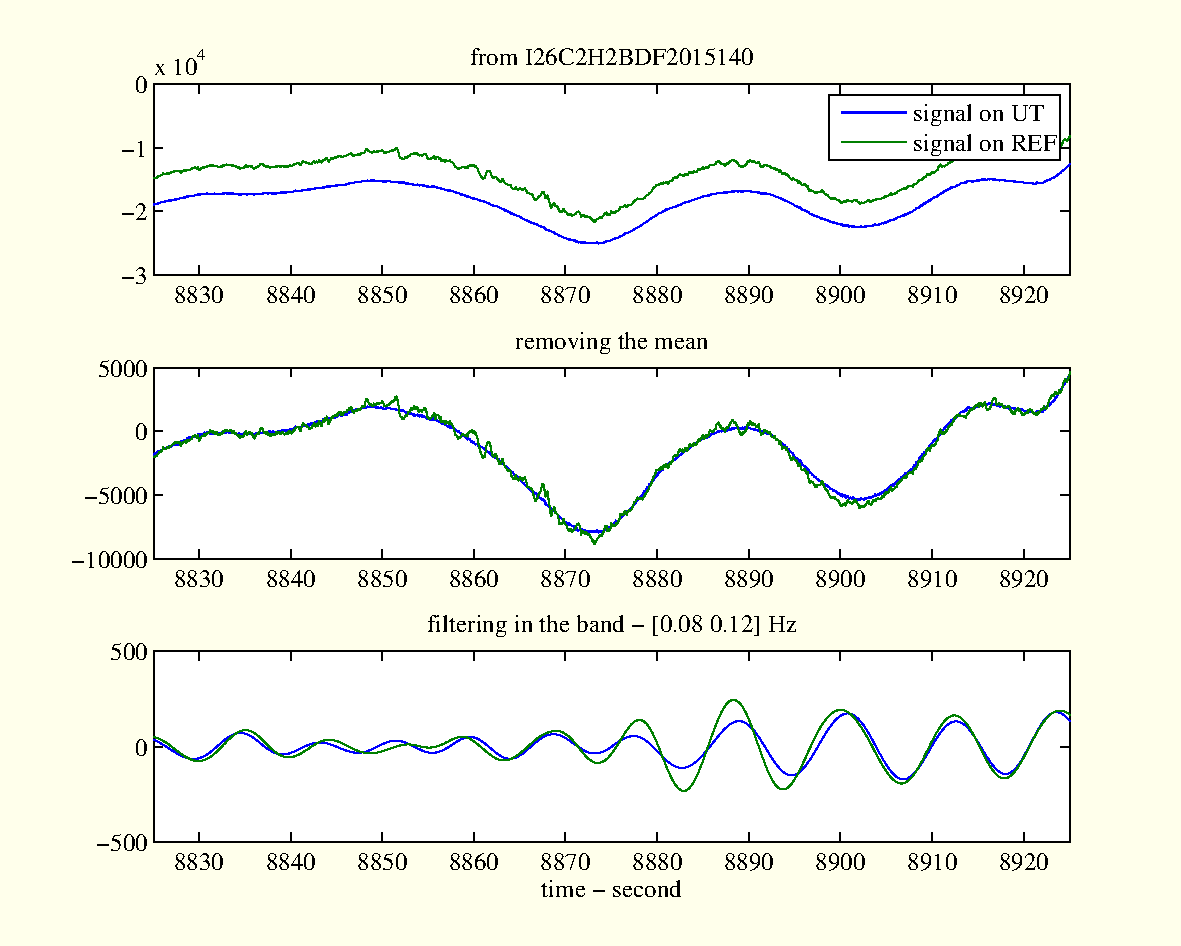
\includegraphics[scale=0.5]{signalsanomaly.pdf}
\end{minipage}
\begin{minipage}[c]{8cm}
              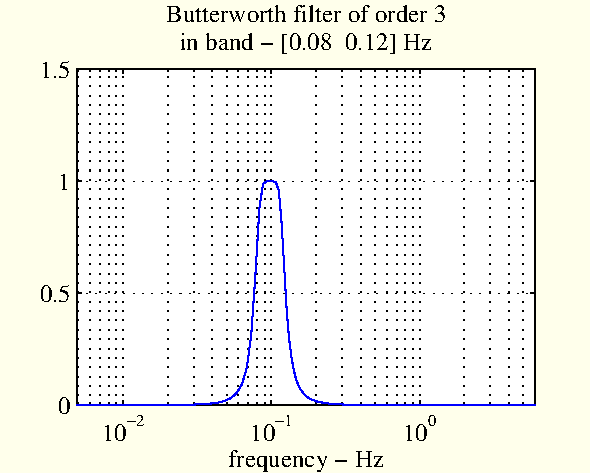
\includegraphics[scale=0.5]{filteranomaly.pdf}    

\end{minipage}
\centering
\caption{Filtered signals}
\label{fig:filteredsignals}
\end{figure}


%===========================================


%===========================================
%===========================================
%===========================================
\chapter{Wind effect on NRS}
\label{chap:windonNRS}
% !TEX root = ../calibreport.tex
%============================================
%============================================
\section{Dip on the curves}
%============================================
In all previous figures we observe an important dip around 0.1 Hz.  Also we have reported figure \ref{fig:afewdays1colocation} the ratio \eqref{eq:ratio-sup-bis-exact} for a few days on the location H2C2. The different colors are for different days. The distribution seems to be uniform and does not depend on the day. The ratio seems to be different of 1.\\*

If the MSC is about 0.99, meaning that the noises on the two sensors are negligible, and if the two sensors have the same response, the only reason to get a ratio less than 1, is that the acoustical SOI on the SUT is attenuated, may due to the noise system reduction. That would write: it exists $\alpha\in\mathbb{C}$ with $|\alpha|<1$ s.t.:
\begin{eqnarray}
\label{eq:model-of-obervation}
\left\{
\renewcommand\arraystretch{1.6}
\begin{array}{rcl}
x_{\ut}(t)&=&g_{\ut}  \star (\alpha s(t))
\\
x_{\rf}(t)&=&g_{\rf}  \star s(t)
\end{array}
\right.
\end{eqnarray}

\figscale{afewdays1colocation.pdf}{a few days on H2C2. Only the band $[0.08-0.12]$ Hz is selected. The coherence is above $0.99$. The different colors for the different days.}{fig:afewdays1colocation}{0.5}

In the following of this chapter we consider a simple wind model leading to a loss of coherence which can explain the dip. 

%Another way to see the response differences between the 2 sensors in the band  $[0.08-0.12]$ Hz (gain ratio different of 1), appears figure \ref{fig:filteredsignals}. A zoom of the signals is plotted. It consists of about 1 minute, around a position where the observed coherence is above $0.99$. We see that the signal on the SREF  is bigger than this on the SUT. There is no way and no reason to reject this time window since the difference can be due either to the loss of gain or a unknown transfer function. 
%\begin{figure}%{20cm}
%\begin{minipage}{10cm}
%              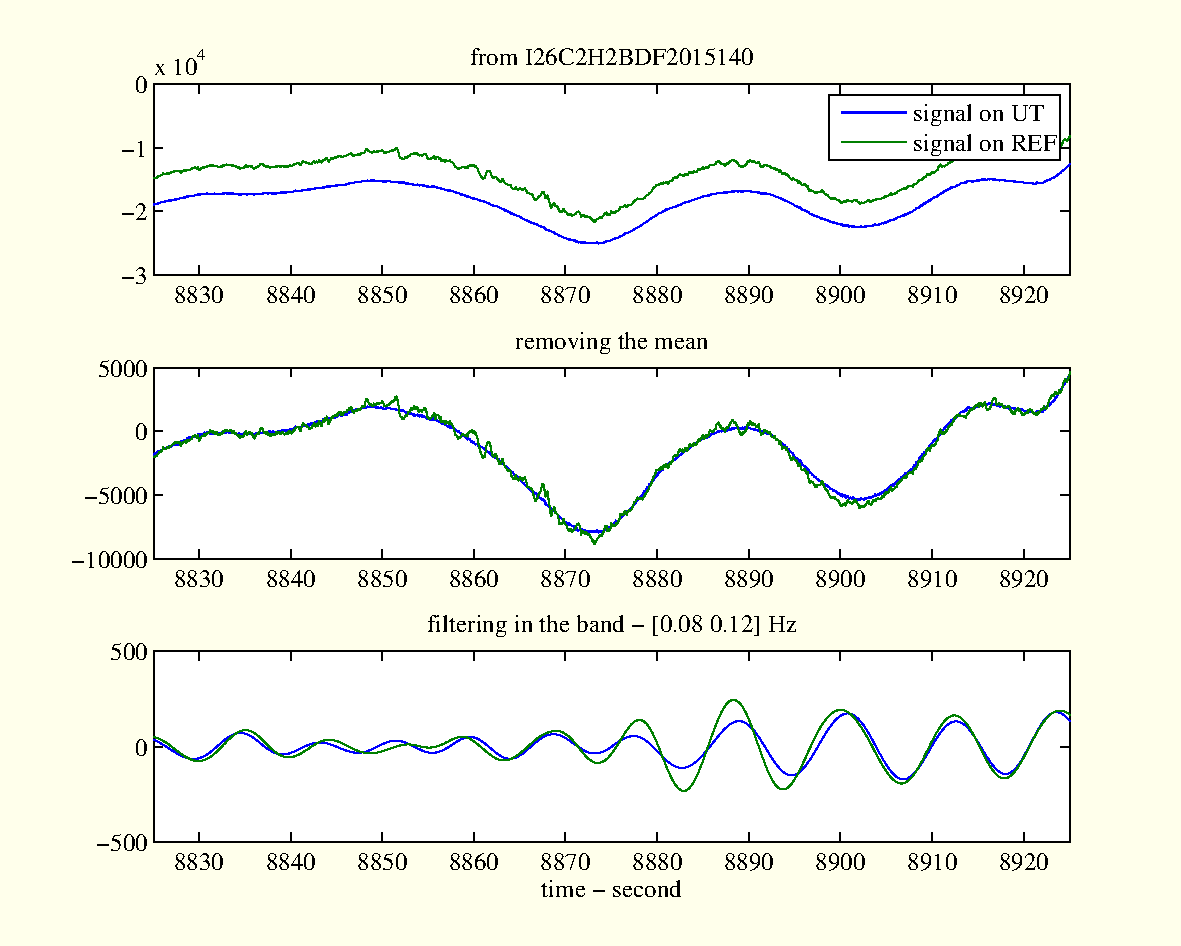
\includegraphics[scale=0.5]{signalsanomaly.pdf}
%\end{minipage}
%\begin{minipage}[c]{8cm}
%              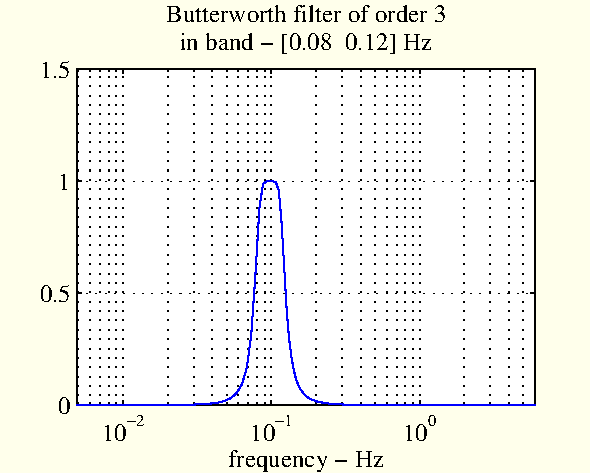
\includegraphics[scale=0.5]{filteranomaly.pdf}    
%
%\end{minipage}
%\centering
%\caption{Filtered signals}
%\label{fig:filteredsignals}
%\end{figure}
%


\clearpage
%============================================
%============================================
\section{Introduction}
%============================================
The noise reduction system (NSR) commonly used in front of the infrasonic sensors in the IMS stations is based on the property that the wind noise appears as spatially uncorrelated at the air inlets of the NRS. Therefore by summation, the SNR is improved in the ratio of the number of inlets. 

Unfortunately this gain is reduced in low frequencies as it has been observed by Alcoverro and al. \cite{alcoverro:2005}. This effect is characterized by the parameter $\zeta=v/f$ where $v$ denotes the wind velocity and $f$ the frequency. $\zeta$ can be interpreted as a ``wavelength'' and must be compared to the inlet inter-distances. If $\zeta$ is of the same order of magnitude of the inter distances, spatial coherence increases. It is not a good news, at first because the noise reduction  is lower. Another drawback occurs when we want to calibrate the sensor by using a second sensor without NRS. In this case the levels of the coherent part will be different and we have no way to identify it.

As a quantitative illustration for wind velocity above $5$ m/s, measurement is no more possible. But for velocity around $1$ m/s and for frequency under $0.01$ Hz, $\zeta>100$ m and the wind is seen as coherent by the full NSR. In the middle range for velocity around $1$ m/s and frequency around $0.1$ Hz, $\zeta\approx 10$ m and a part of the wind noise is seen as coherent just because the NRS. That can induce artefact in the {\it in-situ} calibration because the coherence level close to 1 does not guaranty that the system to solve is well determined.


This article proposes a model for the spatial coherency, as it observed in \cite{alcoverro:2005} and presents simulated and experimental results. This model is similar to the model proposed in \cite{nouvellet_itwb:2013} which is derived from the pioneer approach of Mack and Flinn \cite{mack_flinn:1971}.

%============================================
%============================================
\section{Model for wind turbulences}
Wind turbulence is a very complex air movement. Here we assume that it can be described (as a gray box) by a stationary random  process whose coherence matrix depends on the distance between two spatial locations. At first we just summarize useful definitions of stationary $M$-ary process.

%============================================
\subsection{Stationary $M$-ary process}
An $M$-ary process $x(t)=\begin{bmatrix}
x_{1}(t)&\ldots&x_{m}(t)&\ldots&x_{M}(t)
\end{bmatrix}^{T}$ is associated to a spatial-time description. More specifically, $t$ denotes the time and $m$ an index associated with the 3D spatial locations, usually related to a sensor array.  Therefore we have to consider spatial and temporal properties. For example, an $M$-ary process could be:
\begin{itemize}
 \item
temporally white, meaning that $\esp{x_m(t)x_m(t')}=0$ for $t\neq t'$,
\item
spatially white, meaning that $\esp{x_m(t)x_{m'}(t)}=0$ for $m\neq m'$.
\end{itemize} 
There is no relationship between these two notions. In the general case $\esp{x_m(t)x_{m'}(t')}$ does depend on $(m,m',t,t')$. Temporal stationarity refers to the property that the statistics do depend on $(t-t')$. Spatial ''stationarity'' is a littlebit more complicate because of the 3D coordinates. In some simple cases $\esp{x_m(t)x_{m'}(t')}$ could depend only on the distance between the 2 points indexed by $m,m'$. A particular case is when $\esp{x_m(t)x_{m'}(t')}=0$ for $m\neq m'$ which is called spatially white.

%============================================
\subsubsection{Spectral description}
When the process is a wide sense stationary (WSS) process  a spectral representation can be associated to the covariances. A zero-mean WSS  process is defined by the property that the covariance matrix $R(h)=\esp{x(t+h)x^{H}(t)}$ does not depend on $t$. It is also characterized by the spectral matrix which is the Fourier transform of the covariance matrix sequence:
\begin{eqnarray}
 \Gamma(f) = \int e^{-2j\pi fh}R(h)dh
\end{eqnarray}
where $\Gamma(f)$ is a square matrix of size $M$.

The most fundamental property says that, for any value of the frequency $f$, the spectral matrix is a non-negative matrix. Moreover if $x(t)$ is real, $\Gamma(f)=\Gamma(-f)$.

If the spectral matrix is of rank 1, the process is said spatially coherent. If the spectral matrix is diagonal we say that the process is spatially white. If the spectral matrix is rank deficient we say that the process is partially-coherent. A process whose spectral matrix $\Gamma(f)=\sigma^{2}I_{M}$ is both spatially and temporally  white, because $\Gamma(f)$ does not depend on $f$.

It is also common to consider the function
\begin{eqnarray}
\label{eq:correlationcoherence}
 C_{km}(f)
 &=&\frac{\Gamma_{km}(f)}{\sqrt{\Gamma_{kk}(f)\Gamma_{mm}(f)}}
\end{eqnarray}
where it is assumed that $\Gamma_{kk}(f)\Gamma_{mm}(f)\neq 0$. We can also use the matricial notation
\begin{eqnarray}
 \label{eq:def-generalMSC}
  C(f) = P^{-1}(f)  \Gamma(f) P^{-1}(f)
\end{eqnarray}
or
\begin{eqnarray}
 \label{eq:reverse-def-generalMSC}
  \Gamma(f) = P(f) C(f) P(f)
\end{eqnarray}
where
\begin{eqnarray}
  \label{eq:spectral-content}
 P(f) =   \begin{bmatrix}
  \Gamma_{11}^{1/2}(f)&0&\cdots&0
  \\
  0&\Gamma_{22}^{1/2}(f)&\cdots&0
  \\
  \vdots
  \\
  0&\cdots&0&\Gamma_{MM}^{1/2}(f)
  \end{bmatrix}
\end{eqnarray}
The $M$-ary matrix
\begin{eqnarray}
 \label{eq:coherence-matrix}
 C(f)=\begin{bmatrix}
1&C_{12}(f)&\ldots\\
C_{21}(f)&1& \ldots\\
\vdots\\
\ldots&\ldots&C_{M,M-1}(f)&1
\end{bmatrix}
\end{eqnarray}
is called the coherence matrix. The  function 
\begin{eqnarray}
 \label{eq:def-coherence-function}
 \MSC_{km}(f)=|C_{km}(f)|^{2}
\end{eqnarray}
is called the magnitude square coherence, in short MSC, between $x_{k}(t)$ and $x_{m}(t)$. 
It is easy to show that $\MSC_{km}(f)\leq 1$ and
\begin{eqnarray}
 \label{eq:rhomlfeq1}
 \MSC_{km}(f)=1,\quad \forall f
\end{eqnarray}
if and only if $x_{k}(t)$ and $x_{m}(t)$ are related by a linear filter. When $\MSC_{km}(f)=1$ for all pairs $(k,m)$ the spectral matrix is of rank $1$, hence 
\begin{eqnarray}
C(f)={\mathds 1}_M{\mathds 1}_M^T
\end{eqnarray}
and the process is fully coherent. 
%================================================================= 
\subsubsection{WSS filtering}
A fundamental property concerns the filtering. Let us consider an $M$-ary zero-mean WSS process $x(t)$ with the spectral matrix $\Gamma_x(f)$. Let $y(t)$ the $N$-ary process on the output of a multiple input multiple output (MIMO) filter whose frequency response is the matrix  $K(f)$ of size $N$ by $M$. Then $y(t)$ is a WSS process with zero-mean and whose the spectral matrix writes:
\begin{eqnarray}
 \label{eq:filteringMIMO}
 \Gamma_y(f)&=&K(f)\Gamma_x(f)K^H(f)
\end{eqnarray}
%================================================================
%================================================================
\subsection{Wind noise model}
%================================================================
Wind turbulence is a very complex air movement. Here we assume that it can be described by a stationary random  process whose coherence matrix as the following entry form \cite{nouvellet_itwb:2013}:
\begin{eqnarray}
\label{eq:sm-general-random}
C_{km}(f) = \int \exp(-2j\pi f (r_k-r_m)^T k ) \,p_K(k)dk
\end{eqnarray}
where $f$ is the frequency, $r_k$ and $r_m$ are any two 3D locations and $k$ the slownwess vector. $p_K(k)$ is a probability distribution in $\mathds{R}^{3}$ meaning that the slownwess vector is considered to be random.
Let assume at first that $k$ is deterministic, that writes $p_{\Delta}(u)du=\delta_{0}(du)$. Hence expression  \eqref{eq:sm-general-random} can be written:
\begin{eqnarray*}
C_{km}(f) = e^{-2j\pi f(r_k-r_m)^Tk_0}
\end{eqnarray*}
That means that the displacement is a plane wave. It is worth to notice that the matrix $C$ can be written:
\begin{eqnarray*}
C(f) = E(f)E^{H}(f), 
\quad\mathrm{with}\quad
E(f) = \begin{bmatrix}
e^{-2j\pi r_{1}^{T} k_0}&\ldots&e^{-2j\pi r_{M}^{T}k_0}
\end{bmatrix}^{T}
\end{eqnarray*}
Hence the multivariate process is fully coherent.

The model, derived from the pioneer work by Mack and Flinn \cite{mack_flinn:1971} for the loss of coherence, considers that the azimuth $a$, the elevation $e$ and velocity $v$ are random variables. More specifically, we assume that the 3D vector $\mu=(a,e,v)$ writes:
\begin{equation}
 \label{eq:randomnesswn}
 \mu=\mu_{0}+\nu
\end{equation} 
where $\mu_{0}=(a_{0},e_{0},v_{0})$ is a deterministic part and $\nu$ a zero-mean Gaussian random vector of dimension 3, whose covariance is denoted $\Sigma_{\mu}$. It is shown in the appendix that:
\begin{eqnarray}
\label{eq:Cfr1r2Gaussian}
C_{m,\ell}(f)=
\underbrace{e^{-2j\pi f(r_{m}-r_{\ell})^{T}k_{0}}}_{\text{pure delay}}
 \underbrace{e^{-2\pi^{2}(f/v_0)^{2}(r_{m}-r_{\ell})^{T}
                 \tilde \Sigma_{k}(r_{m}-r_{\ell})}}_{\text{coherence effect}}
 \end{eqnarray}
where $\tilde \Sigma_{k}$ is given by \eqref{eq:aec2theta}. We let $\zeta=v_0/f$ that appears as a ``wavelength''. Using the MSC definition \eqref{eq:def-coherence-function}  we derive the following expression:
\begin{eqnarray}
\label{eq:MSCwind}
\MSC_{km}(f)=
e^{-4\pi^{2}(r_{m}-r_{\ell})^{T}
                 \tilde \Sigma_{k}(r_{m}-r_{\ell})/\zeta^{2}}
 \end{eqnarray}

The same parameter $\zeta$ has been proposed by Alcoverro and al. in \cite{alcoverro:2005} to characterize the coherence of the wind disturbances for closely located sensors. The expression \eqref{eq:MSCwind} has a clear meaning: the coherence  between any two spatial locations decreases when the distance between them is large compared to the ''wavelength'' $\zeta$. 

It follows that when $\zeta$ is low, i.e. low wind velocity and/or high frequency, the wind signals on the different air inlets are almost uncorrelated hence $M$ works as a reduction factor. On the other hand when $\zeta$ is high, i.e. high wind velocity and/or low frequency, the wind signals on the different air inlets are strongly correlated hence that allows good conditions to estimate the ratio between the sensor responses. In the mid-range, it appears that the common signal is present with two different amplitudes on the two sensors inducing a ratio different from $1$. Simulation below gives an illustration of that.




%============================================
\subsection{Coherence level as a function of $v/d$}

To show that our model is in good agreement with the experimental results reported in  \cite{alcoverro:2005} we  consider the following simulation: we choose $M$ random locations in such a way we obtain several different inter-distances. Using the formula \eqref{eq:Cfr1r2Gaussian} we compute for each pair of locations the frequency $f_{c}$ associated with the coherence level of $0.5$. This value has been chosen in  \cite{alcoverro:2005} to define a cut-off for the MSC. We also compute the ratio $v/d$ where $d$ is the distance between the two locations. Finally the coordinate couples $(v/d,f_{c})$ are reported figure \ref{fig:f05asvond}. The obtained cloud shape figure is very similar to the observation values reported in
figure 5 of \cite{alcoverro:2005}. It is worth to notice that the frequency $f_{c}$ does not depend only on the distance. The reason is the coherence formula depends on the quadratic form $(r_m-r_k)^{T}\tilde \Sigma_{k}(r_m-r_k)$ and therefore on the angle between $(r_m-r_k)$ and the  eigenvectors of the matrix  $\tilde \Sigma_{k}$. This quadratic form reduces to the euclidian distance if $\tilde \Sigma_{k}\propto I_{3}$. 
 \figscale{f05asvond.pdf}{Frequency $f_c$ associated with the MSC level $0.5$ as a function of $v/d$. }{fig:f05asvond}{0.8}


 \newpage
%======================================================
%======================================================
 \section{Application to the {\it in-situ} calibration method}
%======================================================
%======================================================
 %\subsubsection{Coherence with/without NRS}
%======================================================



	We consider a sensor with its NRS. This sensor is called sensor under test (SUT). We also consider an other sensor with no NRS, representing the reference sensor (Sref). The NRS consists  of $M=96$ air identical inlets located at the ends of pipes. The scheme is reported on the figure \ref{fig:bigschema}. Thanks to the  Gabrielson's study \cite{gabrielson:2011}, the transfer function $U(f)$ between any inlet and the cavity center of the NRS can be performed as a function of the geometrical structure of the NRS.
% and the transfer function $H(f)$ associated to the reference sensor can be performed. 
%Calculation algorithm for the reference sensor gives $H(f)\approx 1$, hence the ratio $G(f)/H(f)\approx G(f)$ in the full frequency band.

\figscale{bigschema.pdf}{$S_{x}(f)$ spectral matrix de dimension $(M+1)$, $S_{y}(f)$ spectral matrix de dimension $2$, $S_{z}(f)$ spectral matrix de dimension $2$}{fig:bigschema}{0.6}

The spectral matrix of the $(M+1)$-ary input signal writes:
\begin{eqnarray}
\label{eq:Sxf}
 S_x(f) = \gamma_{s}(f) \mathds{1}_{M+1}\mathds{1}_{M+1}^T+ \Gamma(f)
\end{eqnarray}
where $\gamma_{s}(f)$ is the spectral density of the coherent part, which is generally acoustic. By acoustic we mean that the wave has a velocity $c$ of the order of magnitude of $300$ m/s. Let us notice that the associated wavelength of this acoustic part is greater  than 75 meter for any frequencies below 4 Hz.

We assume that the spectral square matrix $\Gamma(f)$, whose size is $(M+1)$, is given by the expression \eqref{eq:reverse-def-generalMSC}  where $C(f)$ entries are given by \eqref{eq:Cfr1r2Gaussian} and 
\begin{eqnarray}
  \label{eq:spectral-content}
 P(f) =   \begin{bmatrix}
  \gamma_{u}^{1/2}(f)&0&\cdots&&0&
  \\
  0&\gamma_{u}^{1/2}(f)&\cdots&&0&
  \\
  \vdots
  \\
  0&\cdots&0&\gamma_{u}^{1/2}(f)&0
  \\
  0&\cdots&&0&\gamma_{r}^{1/2}(f)
  \end{bmatrix}
\end{eqnarray}
Here it is assumed that the noise has the same level $\gamma_{u}(f)$ on all NRS inlets but is different on the reference sensor denoted $\gamma_{r}(f)$.

It follows that the $2\times 2$ spectral matrix associated to the signals at the inputs of the two sensors writes:
\begin{eqnarray}
\label{eq:Syf}
 S_y(f) = K(f) S_x(f) K^H(f)
 \end{eqnarray}
where
\begin{eqnarray*}
K(f)&=&
\begin{bmatrix}
U_{1}^*(f)&\ldots&U_{M}^*(f)&0
\\
0&\ldots&0&1
\end{bmatrix}
\end{eqnarray*}
where we assume that the transfer function of the pipe of the reference sensor is $1$. 

In the following we assume that $U_{1}(f)=\cdots= U_{M}(f)=U(f)$.

From \eqref{eq:Syf} we derive that:
\begin{eqnarray*}
\label{eq:Syentries}
S_{y,11}(f)&=&
|U(f)|^2 \, (M^2\gamma_{s}(f) + \gamma_{u}(f) S_M(f))
\\
S_{y,22}(f)&=&(\gamma_{s}(f) +\gamma_{r}(f))
\\
S_{y,12}(f)&=&
U^{*}(f)\, (M\gamma_{s}(f)+\gamma_{u}^{1/2}(f)\gamma_{r}^{1/2}(f)s_M(f))
\\
S_{y,21}(f)&=&S_{y,12}^{*}(f)
\end{eqnarray*}
where
\begin{eqnarray*}
 S_M(f) =\sum_{k=1}^{M}\sum_{k'=1}^{M}C_{k,k'}
&\mathrm{and}&
 s_M(f) =\sum_{k=1}^{M}C_{k,M+1}
\end{eqnarray*}
Let us notice that for small values of $\zeta$, the $(M+1)$ entries are spatially uncorrelated hence $C$ is the identity leading to
$S_M(f)=M$ and $s_M(f) =0$.

We denote 
\begin{eqnarray*}
S_{z}(f)&=&
\begin{bmatrix}
S_{UU}(f)&S_{UR}(f)
\\
S_{RU}(f)&S_{RR}(f)
\end{bmatrix}
\end{eqnarray*}
with
\begin{eqnarray}
\label{eq:Syentries}
S_{UU}(f)&=& |G_{u}(f)|^2 \,|U(f)|^2 \, (M^2 \gamma_{s}(f)+ \gamma_{u}(f) S_M(f))
\\
S_{RR}(f)&=&|G_{r}(f)|^2 (\gamma_{s}(f)+\gamma_{r}(f))
\\
S_{UR}(f)&=& G_{u}(f)G_{r}^{*}(f)U^{*}(f)\, 
   (M\gamma_{s}(f)+\gamma_{u}^{1/2}(f)\gamma_{r}^{1/2}(f)s_M(f))
\\
S_{RU}(f)&=&S_{UR}^{*}(f)
\end{eqnarray}
Let us remark that a perfect NRS would have $U(f)=1/M$ for all frequencies. Unfortunately that is not satisfied for high frequency values. Indeed it is known that the NRS presents a resonance above $2$ Hz.

At first  if we consider that $U(f)=1/M$, $S_M(f)=M$ and $s_{M}(f)=0$ then we obtain
\begin{eqnarray}
\label{eq:Syentries-idealcase}
S_{UU}(f)&=& |G_{u}(f)|^2  (\gamma_{s}(f)+ \gamma_{u}(f) /M)
\\
S_{RR}(f)&=&|G_{r}(f)|^2 (\gamma_{s}(f)+\gamma_{r}(f))
\\
S_{UR}(f)&=& G_{u}(f)G_{r}^{*}(f) \gamma_{s}(f)
\\
S_{RU}(f)&=&S_{UR}^{*}(f)
\end{eqnarray}
We recognize the classical expression which is the base of the {\it in-situ} calibration. We see also that the noise level is divided by $M$ which is what we expect using an NRS. Unfortunately, since  this ratio $\gamma_{u}(f)/\gamma_{r}(f)$ is unknown, the system is underdetermined. One way to circumvent  this problem is to consider that the wind noises are very close to zero. Indeed if $\gamma_{u}(f)=\gamma_{r}(f)=0$
\begin{eqnarray*}
 G_{u}(f) &=& \frac{S_{UU}(f)}{S_{RU}(f)}\, G_{r}(f)
\end{eqnarray*}


To test the zero-noise it is well-known that the MSC can be used but we have to keep in mind that the MSC equal 1 does not mean that the ratio between the sensor response is 1. It only means that the ratio is a transfer function as for example a pure number. It is the reason why the ratio presents a dip as we see below.

%==================================================================
\subsubsection{MSC}
%==================================================================
In this section we show that the MSC could be very close to 1 and the sensor frequency response ratio is not equal to 1. The MSC successively writes:
\begin{eqnarray}
\label{eq:RsuponM}
 \MSC(f) &=& \frac{|S_{UR}(f)|^2}{S_{UU}(f)S_{RR}(f)} \nonumber
 \\
 &=& \frac{|M\gamma_{s}(f)+\gamma_{u}^{1/2}(f)\gamma_{r}^{1/2}(f)s_M(f))|^2}
    {(M^2 \gamma_{s}(f)+ \gamma_{u}(f) S_M(f))(\gamma_{s}(f)+\gamma_{r}(f))}
\end{eqnarray}
We let $\rho_{i}(f)=\gamma_{i}(f)/\gamma_{s}(f)$. Then
\begin{eqnarray}
\label{eq:RsuponM-rho}
 \MSC(f) 
 &=& \frac{|M+\rho_{u}^{1/2}(f)\rho_{r}^{1/2}(f)s_M(f))|^2}
    {(M^2 + \rho_{u}(f) S_M(f))(1+\rho_{r}(f))}
\end{eqnarray}
It follows:
\begin{itemize}
 \item
For high frequencies $s_M(f)\approx 0$ and $S_M(f)\approx M$, hence 
\begin{eqnarray}
\label{eq:MSCHF}
 \MSC(f) 
 \approx \frac{1}{(1+\rho_{u}(f)/M)(1+\rho_{r}(f))}
\end{eqnarray}

 \item
For very low frequencies $s_M(f)= M$ and $S_M(f)= M^2$, hence:
\begin{eqnarray}
\label{eq:MSCBF}
 \MSC(f) = \frac{(1+\sqrt{\rho_{u}(f)\rho_{r}(f)})^{2}}{(1+\rho_{u}(f))(1+\rho_{r}(f))}
\end{eqnarray}
	the MSC could be close to $1$ even if $\rho_{u}(f)$ and $\rho_{r}(f)$ are different of 0.
 \item
For mid-range, $s_M(f)\approx \lambda_1 M$ and $S_M(f)\approx \lambda_2 M^{2}$, hence 
\begin{eqnarray}
\label{eq:MSCMidF}
 \MSC(f) \approx 
    \frac{(1+\lambda_{1}\sqrt{\rho_{u}(f)\rho_{r}(f)})^{2}}
           {(1+\lambda_{2} \rho_{u}(f))(1+\rho_{r}(f))}
\end{eqnarray}
If $\lambda_{1}$ and $\lambda_{2}$ are close to $1$, the MSC could be close to $1$ even with $\rho_{i}(f)\neq 0$.
\end{itemize}
In conclusion $\MSC(f)$ close to $1$ does not mean that  $\rho_{u}(f)$ and $\rho_{r}(f)$ are close to 0 and in this case the system is still underdetermined.



\newpage\clearpage
%==================================================================
\subsubsection{Frequency response ratio}
%==================================================================
Assuming that $U(f)=1/M$ for all frequencies, the frequency response ratio writes:
\begin{eqnarray*}
R(f)&=& 
\frac{S_{UU}(f)}{S_{UR}^{*}(f)}=\frac{ G_{u}(f)}{G_{r}(f)}\times
\frac{ 1+ \gamma_{u}(f) S_M(f)/M^{2} \gamma_{s}(f)}{
   1+\gamma_{u}^{1/2}(f)\gamma_{r}^{1/2}(f)s_M(f)/M \gamma_{s}(f)}
\end{eqnarray*}
if $\gamma_{u}(f) =\gamma_{r}(f) =1$, and $\gamma_{u}(f) =\rho\gamma_{s}(f)$:
\begin{eqnarray*}
R(f)&=& 
\frac{S_{UU}(f)}{S_{UR}^{*}(f)}=\frac{ G_{u}(f)/M}{G_{r}(f)}\times
\frac{M^{2}+ \rho S_M(f)}{M+ \rho s_M(f)}
\end{eqnarray*}
where the quantity $G_{u}(f)/M$ is provided by the Gabrielsson analysis and is very close to $1/M$, except above 2 Hz, due to the resonance effect. Numerical results are reported figure \ref{fig:GonH} for a given shape of $\rho(f)$.


  \figscale{GonH.pdf}{The top curve represents the spectral ratio $\rho(f)$. The two following curves report the magnitude and the phase of the ratio
   The blue parts of   corresponding to an MSC greater than $0.95$. For frequencies over $0.4$ Hz up to $4$ Hz and for low noise levels, the curves reproduce the response of the NRS. In particular on the high frequency part the curves are related to a known resonance effect. For frequencies under $0.08$ Hz and even for low values of $\SNR$, the coherence is very high, because the wind turbulences appear as spatially coherent. In the mid frequency range we can have simultaneously a high MSC and a ratio less than $1$.}{fig:GonH}{0.7}
  
%==================================================================
\newpage\clearpage
%==================================================================
\section{Results in I26}
%==================================================================

\figscale{twospeeds}{Top figure: averaging of the wind speed on plain curve, standard deviation 
around the averaging in dotted curve. Markers indicate the two parts of interest. 
Bottom figure: curves associated to the two parts of interest. The shift between them has a ratio of about $4$ which is about the ratio of the speed means od the  two parts of interest.}{fig:twospeeds}{0.8}

\figscale{twospeedsbis}{see figure \ref{fig:twospeeds}}{fig:twospeedsbis}{0.7}

\figscale{twospeedster}{see figure \ref{fig:twospeeds}}{fig:twospeedster}{0.7}


%===========================================

%===========================================
%===========================================
%===========================================
\chapter{Full process}
\label{chap:fullprocess}
% !TEX root = ../calibreport.tex


%================================
\section{3 programs for test}
The full process consists of
\begin{enumerate}
\item
 move data from the IDC, using {\tt RUNextractfromDB.m}. The data with Matlab format is saved. This data consists of a structure called {\tt records} with the following items:
 \begin{itemize}
 \item
{\tt data}: sequence of samples,
 \item
{\tt Fs\_Hz}: sampling frequency,
\item
{\tt stime}, {\tt time}: start and end times, 
\item
{\tt station}: I26C1--I26C8 or I26H1--I26H8
\item
{\tt channel}: 'BDF' or 'LKO' or 'LWD' or 'LWS'
 \end{itemize}   
Typically in the following we use BDF on H and C.   The three other channels are only provided on H1. Channel LWD yields  the wind speed measurement. The wind sensor is located at about 2 meters above the infrasonic sensor. The frequency sampling depends on the channel. Typically for infrasound signals, the frequency sampling is $20$ Hz, and for wind features is 1 Hz.
    
\item
 using the filtercharacteristics, saved in {\tt filtercharacteristics.mat} and the directory which contains the data from one of the 8 channels, run the program {\tt estimationwithFB.m}. This program saves the useful elements for a display in a selected directory.
 \item
 to display run the program {\tt displaySUTresponse.m} for the file recorded in the selected directory of the previous item.
\end{enumerate}


%================================
\section{Input of the function {\tt fbankanalysis.m}}
\begin{itemize}
\item
signals: an array of size $N\times 2$ where $N$ is a number of samples, the first column is the signal from the SUT channel and the second for the SREF channel,
\item
filter bank settings: see section \ref{sss:filter-bank-settings},
\item
$F_s$: sampling frequency in Hz, typically $20$ Hz,
\item
MSC threshold: threshold for the MSC, typically $0.98$
\end{itemize}
\subsubsection{Summary of the filter bank settings}

\label{sss:filter-bank-settings}

\begin{center}
{\small\verbatiminput{filtercharacteristicsEXAMPLE.m}}
\end{center}

\begin{itemize}
\item
{\tt designname} means that the name of the filter model. The Butterworth model is available in Matlab. 
\item
{\tt Norder} denotes the order of the filter. If 0 there is no filtering. 
\item
{\tt Wlow\_Hz} denotes the low bound in Hz of the filter design,
\item
{\tt Whigh\_Hz} denotes the high bound in Hz of the filter design,
\item
{\tt windowshape} denotes the weighted window. Many windows are available in Matlab. Window is used to do a compromise between the leakage and the bias. Hann's window is commonly used.
\item
{\tt SCPperiod\_sec} denotes the time duration expressed in second of the window used for the spectral estimation,
\item
{\tt overlapDFT} overlapping rate for the spectral estimation,
\item
{\tt overlapSCP} overlapping rate for the different spectral estimates,
\item
{\tt ratioDFT2SCP} is an integer which denotes the ratio between the duration of the spectral estimation window and the duration of the DFT window. 

\end{itemize}


%================================
\section{Output of the function {\tt fbankanalysis.m}}

\begin{verbatim}
% 1) SUTs: structures P x 1
%         xx.estimRsup: Rsup ratio
%         xx.estimRinf: Rinf ratio
%         xx.allMSCs: allMSCs;
%         xx.Nsupthreshold: count of the number of values over
%                   the threshold
%         xx.Nsupthresholdintheband: counts of the number of values
%                   over the threshold in the filter bandwidth
%         xx.frqsFFT_Hz: cell P x 1, each cell consists of
%                   frequency list in Hz of the DFTs
%         xx.SCP = all spectral components
%         xx.indexinsidefreqband = P x 1, indices of the
%                    frequency bounds of each filter
%                    in the xx.frqsFFT_Hz
% 2) filteredsignals, 
% 3) allfrqsFFT_Hz, cell P x 1, each cell for each bank filter consists of
%             frequency list in Hz of the DFTs
% 4) alltimes_sec: cell  Px 1, each cell consists of the structure
%             yy.FFT:     time list in second of the DFTs
%             yy.SD:      time list in second of the SCPs
%             yy.signals: time list in second of the signals
% 5) filterbank



\end{verbatim}




%===========================================

%===========================================
%===========================================
%===========================================
%===========================================
\part{Annexes}
\chapter{Confidence interval on the mean}

% !TEX root = ../calibreport.tex
%==============================================================


We consider a sequence of $N$ data modeled as $N$ i.i.d. r.v. denoted $X_{n}$. An estimator of the mean is given by
\begin{eqnarray*}
\hat \mu_{N} &=&\frac{1}{N}\sum_{n=1}^{N}X_{n}
\end{eqnarray*}
We let
\begin{eqnarray*}
\hat\sigma_{N}^{2} &=& \frac{1}{N-1}\sum_{n=1}^{N}(X_{n}-\hat \mu)^{2}
\end{eqnarray*}
To provide a confidence interval (CI) for $\hat\mu_{N}$ we have
\begin{itemize}
\item
if $X_{n}$ are gaussian with mean $\mu$ and variance $\sigma^{2}$ both unknown, it is show that the CI can be derived from the law of Student with $N-1$ d.o.f. more specifically we have:
\begin{eqnarray*}
\frac{\sqrt{N}(\hat \mu_{N} -\mu)}{\hat\sigma_{N}}&\sim&T_{N-1}
\end{eqnarray*}
leading to the CI:
\begin{eqnarray*}
\hat\mu_{N}-\alpha\frac{\hat\sigma_{N}}{\sqrt{N}}
&
 \leq\mu\leq
&
\hat\mu_{N}+\alpha\frac{\hat\sigma_{N}}{\sqrt{N}}
\end{eqnarray*}

\item
for large $N$ (limit central theorem), it is shown that 
\begin{eqnarray*}
\frac{\hat\sigma_{N}}{\sqrt{N}}
\end{eqnarray*}
leading to the CI:
\begin{eqnarray*}
\hat\mu_{N}-\beta\frac{\hat\sigma_{N}}{\sqrt{N}}
&
 \leq\mu\leq
&
\hat\mu_{N}+\beta\frac{\hat\sigma_{N}}{\sqrt{N}}
\end{eqnarray*}

\item
for limit central theorem, 

\end{itemize}
%===========================================
\chapter{Wide sense stationary process}
\label{ann:wss}
% !TEX root = ../calibreport.tex
%==============================================================
A multivariate time series $x_{n}$ is said to be a zero-mean wide-sense stationary (WSS) process of second order iif $\esp{x_{n}}=0$, $\trace{\esp{x_{n}x_{n}^{H}}}<+\infty$ and the sequence of covariance matrices\footnote{The superscript $H$ denotes the transposition-conjugaison, $T$ the transposition and $*$ the conjugaison.} $R(h)=\esp{x_{n+h}x_{n}^{H}}$ does not depend on $n$. 
It follows that $R(h)=R^{H}(-h)$. Therefore if $x_{n}$ is real $R(h)=R^{T}(-h)$.

Under very general conditions, its Fourier transform
$$
 \Gamma(f)=\sum_{h} R(h)e^{-2j\pi hf},\quad\text{with}\quad 
 f\in(0,1)
$$
exists which is called the spectral matrix sequence. A fundamental property says that 
$$
 \forall f, \quad \Gamma(f)\geq 0
$$
The non-negativity of $\Gamma(f)$ implies that $\Gamma_{ij}(f)=\Gamma_{ji}^{*}(f)$ and $\Gamma_{ii}(f)\geq 0$. If $x_{n}$ is real alors $\Gamma(f)=\Gamma(-f)$. For example for a bivariate process we have
$$
 \Gamma(f)=
 \begin{bmatrix}
 \Gamma_{11}(f)&\Gamma_{12}(f)\\
 \Gamma_{21}(f)&\Gamma_{22}(f)
 \end{bmatrix}
$$
where $ \Gamma_{11}(f)$ and $ \Gamma_{22}(f)$ are both positive functions. The coherence matrix is defined by
\begin{eqnarray*}
 C(f) 
 &=&
 \begin{bmatrix}
 \Gamma_{11}^{-1/2}(f)&0
 \\
 0& \Gamma_{22}^{-1/2}(f)
 \end{bmatrix}
  \begin{bmatrix}
 \Gamma_{11}(f)&\Gamma_{12}(f)\\ \Gamma_{21}(f)&\Gamma_{22}(f)
 \end{bmatrix}
 \begin{bmatrix}
 \Gamma_{11}^{-1/2}(f)&0
 \\
 0& \Gamma_{22}^{-1/2}(f)
 \end{bmatrix}
 \\
 &=&
   \begin{bmatrix}
 1&C_{12}(f)\\ C_{21}(f)&1
 \end{bmatrix}
\end{eqnarray*}
with $C_{12}(f)=C_{2,1}^{*}(f)$. Let
\begin{eqnarray}
\label{eq:defCSD}
 \eta_{12}(f)= \frac{\Gamma_{12}(f)}{\sqrt{\Gamma_{11}(f)\Gamma_{22}(f)}}
\end{eqnarray}
which is called the  normalized cross spectral density and
\begin{eqnarray}
\label{eq:defMSC}
 \MSC(f)= \frac{|\Gamma_{12}(f)|^{2}}{\Gamma_{11}(f)\Gamma_{22}(f)}
\end{eqnarray}
which is called the Magnitude Squared Coherence (MSC) or shortly the coherence. A fundamental property says that 
$$
 \forall f, \quad \MSC(f)\leq 1
$$
and the equality occurs iff it exists a filter s.t. one signal of the bivariate process is the filtering  of the other. In this case $\Gamma(f)$ is, up to a a multiplicative positive value, a projector of rank 1. A fundamental example is given by
$$
\begin{array}{ccc}
\left\{
 \begin{array}{rcl}
 x_{1,n}&=&g_{1,n}\star s_{n}
 \\
 x_{2,n}&=&g_{2,n}\star s_{n}
\end{array}
\right.
&\Leftrightarrow&
x_{n}=\begin{bmatrix}
x_{1,n}\\ x_{2,n} 
\end{bmatrix} = h_{n} \star s_{n}
\end{array}
$$
where $s_{n}$ is a monovariate WSS process with spectral density $\gamma_{s}(f)$. Then the spectral matrix of the bivariate process writes 
$$
 \Gamma(f)=\gamma_{s}(f)G(f)G^{H}(f)
$$
and
$$
C(f) 
= \begin{bmatrix}1&1\\1&1\end{bmatrix}
= \begin{bmatrix}1\\1\end{bmatrix}
  \begin{bmatrix}1&1\end{bmatrix}
$$
In the noisy case if the spectral matrix of the two noises is diagonal with respective spectral densities $\gamma_{1}(f)$ and  $\gamma_{2}(f)$, the spectral matrix writes:
$$
 \Gamma(f) = \gamma_{s}(f)
 \renewcommand\arraystretch{1.6}
 \begin{bmatrix}
| G_{1}(f)|^{2}& G_{1}(f)G_{2}^{*}(f)
 \\
 G_{1}^{*}(f)G_{2}(f)& | G_{2}(f)|^{2}
 \end{bmatrix}
 +
  \begin{bmatrix}
 \gamma_{1}(f)| G_{1}(f)|^{2}& 0
 \\
 0& \gamma_{2}(f)| G_{2}(f)|^{2}
 \end{bmatrix}
$$
then
\begin{eqnarray*}
 \MSC(f) 
 &=& 
 \frac{|\Gamma_{1,2}(f)|^{2}}{\Gamma_{1,1}(f)\Gamma_{2,2}(f)}
 \\
 &=&
 \frac{1}
   {(1+\mathrm{SNR}_{1}^{-1}(f))(1+\mathrm{SNR}_{2}^{-1}(f))}
\end{eqnarray*}
where
$$
 \mathrm{SNR}_{1}(f)=\frac{\gamma_{s}(f)}{\gamma_{1}(f)}
 \quad\text{and}\quad
 \mathrm{SNR}_{2}(f)=\frac{\gamma_{s}(f)}{\gamma_{2}(f)}
$$

All these expressions can be generalized for more than 2 dimensions.

\chapter{Theoretical results on spectral estimation}
\label{ann:spectral-estimation}
 % !TEX root = ../calibreport.tex
%==============================================================
%==============================================================
\section{Non parametrical spectral estimation}
%==============================================================
Let us consider $x_{n=0:N-1}$ $N$ successive values of a real WSS bivariate process with zero-mean and spectral matrix $\Gamma(f)$. Its DFT writes
$$
 X_{k}=\frac{1}{\sqrt{N}}\sum_{n=0}^{N-1}x_{n}e^{-2j\pi kn/N}
$$
It can be shown that, for large $N$, and for $k\neq 0$ and $k\neq N/2$:
$$
 X_{k}\simiid\mathcal{N}_{c}(0,\Gamma_{k})
$$
where $\Gamma_{k}=\Gamma(k/N)$ and where $\mathcal{N}_{c}$ denotes the complex circular gaussian distribution. The periodogram is defined by 
$$
 P_{k}=X_{k}X_{k}^{H}
$$
In the following section \ref{ann:peridogramproperties}, it is shown that the expectation of the periodogram $P_{k}$ is $\Gamma_{k}$, but unfortunately the dispersion around $\Gamma_{k}$ never goes to 0 when $N$ goes to infinity. The periodogram is not a consistent estimate of $\Gamma_{k}$. A fundamental way to have consistency is to smooth the periodogram (smoothed peridogram). An other approach consists to segment the data in $(2M+1)$ $50\%$-overlapping blocks and averaging the $2M+1$ periodograms, applying a window on each block. That is called Welch's approach in the literature. The 2 approaches are very similar.

For the smoothed periodogram estimator at any frequency $f$ writes: 
\begin{eqnarray}
 \label{eq:smoothedperiodogram}
  \widehat{\Gamma}_{k}=\sum_{m=0}^{2M}W_{m}P_{k-M+m}
\end{eqnarray}
where $k$ is an integer s.t. $\frac{k-1/2}{N}\leq f < \frac{k+1/2}{N}$. That leads to a mean square error (MSE) that writes
\begin{eqnarray}
\label{eq:MSEk}
 \mathrm{MSE}_{k}
 &=&
 \mathcal{G}_{k}+\mathcal{B}_{k}\mathcal{B}_{k}^{H}
\end{eqnarray}
where the bias
\begin{eqnarray}
\label{eq:biassmoothperiodogram}
 \mathcal{B}_{k}= \Gamma_{k}-\sum_{k=0}^{2M}W_{m}\Gamma_{k-M+m}
\end{eqnarray}
and the covariance
\begin{eqnarray}
\label{eq:varGammak}
 \mathcal{G}_{k}= \sum_{k=0}^{2M}W_{m}^{2}
 \diag{\Gamma_{k-M+m}}\diag{\Gamma_{k-M+m}}^{H}
\end{eqnarray}
The choice of the window and its length results from a compromise between bias and variance. Unfortunately this compromise is related to the shape of the spectrum which is \emph{unknown}. Using \eqref{eq:MSEk} we derive a confidence interval replacing deterministic values by their estimates and assuming a gaussian distribution.


%================================================
\section{More periodogram properties}
\label{ann:peridogramproperties}
%================================================
Let us consider $x_{n=0:N-1}$ a sequence of $N$ consecutive values of a real wide-sense stationary bivariate process with zero-mean and spectral matrix $\Gamma(f)$. An fundamental property says that $\Gamma(f)\geq 0$ for any value of $f$. The DFT of the sequence writes
$$
 X_{k}=\frac{1}{\sqrt{N}}\sum_{n=0}^{N-1}x_{n}e^{-2j\pi kn/N}
$$
It can be shown that, for large $N$, and for $k\neq 0$ and $k\neq N/2$:
$$
 X_{k}\simiid\mathcal{N}_{c}(0,\Gamma_{k})
$$
where $\Gamma_{k}=\Gamma(k/N)$ and where $\mathcal{N}_{c}$ denotes the complex circular gaussian distribution whose the probability density writes:
$$
 p_{X_{k}}(x_{k}) = \frac{1}{\pi^{2} |\Gamma_{k}|}e^{-x_{k}^{H}\Gamma_{k}^{-1}x_{k}}
$$
Recall that for any complex gaussian random vector with zero-mean and covariance $\Gamma$ 
we have by definition:
$$
 \esp{XX^{H}} = \Gamma
$$
and
$$
 \esp{XX^{T}} = 0
$$
and if $X_{1\cdots 4}$ denote 4 gaussian complex zero-mean r.v., we have
\begin{eqnarray}
\label{eq:4moment}
\esp{X_{1}^{\beta_{1}}X_{2}^{\beta_{2}}X_{3}^{\beta_{3}}X_{4}^{\beta_{4}}}
&=&
 \esp{X_{1}^{\beta_{1}}X_{2}^{\beta_{2}}}\esp{X_{3}^{\beta_{3}}X_{4}^{\beta_{4}}}
\\
&& +\nonumber
 \esp{X_{1}^{\beta_{1}}X_{3}^{\beta_{3}}}\esp{X_{2}^{\beta_{2}}X_{4}^{\beta_{4}}}
 +
 \esp{X_{1}^{\beta_{1}}X_{4}^{\beta_{4}}}\esp{X_{2}^{\beta_{2}}X_{3}^{\beta_{3}}}
\end{eqnarray}
where $\beta_{i}$ is either ``star'' or ``not-star''.

The formula \eqref{eq:4moment} is very useful to perform the second order moments of the periodogram defined by 
\begin{eqnarray}
\label{eq:defperiodogram}
   P_{k}=X_{k}X_{k}^{H}=\begin{bmatrix}
   X_{1}X_{1}^{*}&X_{1}X_{2}^{*}
   \\
   X_{1}^{*}X_{2}&X_{2}X_{2}^{*}
   \end{bmatrix}
\end{eqnarray}
Let us remark that if we multiply $X_{1}$ and $X_{2}$ by $e^{j\theta}$ the matrix $P_{k}$ is unchanged. Then given $P_{k}$ we can determine $X_{1}$ and $X_{2}$ up to a constant of modulus 1.
It is possible to derive the distributions of $P_{k}$ entries from the distribution of $X_{k}$.
Alleviating the notations by omitting the index $k$, the distribution of these two complex r.v. $X_{1}$, and $X_{2}$ writes
\begin{eqnarray*}
 p_{X_{1},X_{2}}(x_{1},x_{2})
 &=&
 \frac{1}{\pi^{2} (\Gamma_{1,1}\Gamma_{2,2}-|\Gamma_{1,2}|^{2})}
 \\
 &&\hspace{-2cm}
 \exp\left(-
 \frac{
 |x_{1}|^{2}\Gamma_{2,2}+|x_{2}|^{2}\Gamma_{1,1}
 -2|x_{1}|\,|x_{2}||\Gamma_{2,1}|\cos(\alpha)}
 {(\Gamma_{1,1}\Gamma_{2,2}-|\Gamma_{1,2}|^{2})}
 \right)
\end{eqnarray*}
where $\alpha = \arg x_{1}-\arg x_{2}-\arg \Gamma_{1,2}$.

In practical cases we often need only the second order moments. %===========================================
\begin{example}[Variance of $P_{1,1,k}$]
Let us recall that $P_{1,1,k}\ge 0$. It comes
$$
\esp{P_{1,1,k}}=\esp{X_{1}X_{1}^{*}}=\Gamma_{1,1}\geq 0
$$
and
$$
\esp{P_{1,1,k}P_{1,1,k}^{*}}=\esp{X_{1,k}X_{1,k}^{*}X_{1,k}^{*}X_{1,k}}
=2\esp{X_{1,k}X_{1,k}^{*}}\esp{X_{1,k}X_{1,k}^{*}}+0=2\Gamma_{1,1,k}^{2}
$$
then
$$
\var{P_{1,1,k}}=\esp{P_{1,1,k}P_{1,1,k}^{*}}-\esp{P_{1,1,k}}\esp{P_{1,1,k}}^{*}
=\Gamma_{1,1,k}^{2}
$$

\end{example}
%===========================================
\begin{example}[Variance of $P_{1,2,k}$]
Consider we want to determine the second order moments of $P_{1,2,k}$ which is complex. It comes
$$
\esp{P_{1,2,k}}=\esp{X_{1,k}X_{2,k}^{*}}=\Gamma_{1,2}
$$
and
\begin{eqnarray*}
\esp{P_{1,2,k}P_{1,2,k}^{*}}&=&\esp{X_{1,k}X_{2,k}^{*}X_{1,k}^{*}X_{2,k}}
\\
 &=&
\esp{X_{1,k}X_{1,k}^{*}}\esp{X_{2,k}X_{2,k}^{*}}+
 \esp{X_{1,k}X_{2,k}^{*}}\esp{X_{2,k}X_{1,k}^{*}}+0
 \\
 &=&
 \Gamma_{1,1,k}\Gamma_{2,2,k}+\Gamma_{1,2}\Gamma_{1,2}^{*}
\end{eqnarray*}
then
$$
\var{P_{1,2,k}}=\esp{P_{1,2,k}P_{1,2,k}^{*}}-\esp{P_{1,2,k}}\esp{P_{1,2,k}^{*}}
=\Gamma_{1,1,k}\Gamma_{2,2,k}
$$
On the other hand
$$
\esp{P_{1,2,k}P_{1,2,k}} = \esp{X_{1}X_{2}^{*}X_{1}X_{2}^{*}}
=
2 \Gamma_{1,2,k}^{2}
$$
which is complex.
\end{example}

%===========================================

\begin{example}
We want to determine the variance of $P_{1,2,k,R}$. To alleviate the notations we omit the index $k$ and  let $G=P_{1,2}$, $G=P_{1,2}$ and $G_{R}=P_{1,2,R}$. Then
\begin{eqnarray*}
 G_{R}&=&\frac{1}{2}(G+G^{*})
\end{eqnarray*}
at first
$$
\esp{G_{R}}=\frac{1}{2}(\Gamma_{1,2}+\Gamma_{1,2}^{*})=\Gamma_{1,2,R}
$$
then
\begin{eqnarray*}
 \esp{G_{R}^{2}}&=& \frac{1}{4}\esp{GG+G^{*}G^{*}+2GG^{*}}
\end{eqnarray*}
at first
\begin{eqnarray*}
\esp{G^{2}} &=& \esp{X_{1}X_{2}^{*}X_{1}X_{2}^{*}}
\\
&=&\esp{X_{1}X_{2}^{*}}\esp{X_{1}X_{2}^{*}}+0+\esp{X_{1}X_{2}^{*}}\esp{X_{1}X_{2}^{*}}
\\
&=&2(\Gamma_{1,2})^{2}
\end{eqnarray*}
similarly
$$
\esp{G^{*}G^{*}}=2(\Gamma_{1,2}^{*})^{2}
$$
and
\begin{eqnarray*}
2\esp{GG^{*}} &=& 2\esp{X_{1}X_{2}^{*}X_{1}^{*}X_{2}}
\\
&=&2|\Gamma_{1,2}|^{2}+2\Gamma_{1,1}\Gamma_{2,2}+0
\end{eqnarray*}
then
\begin{eqnarray*}
 \var{G_{1,2,R}}
 &=&
 \underbrace{\frac{1}{2}(\Gamma_{1,2})^{2}+\frac{1}{2}(\Gamma_{1,2}^{*})^{2}}
 _{\Gamma_{1,2,R}^{2}-\Gamma_{1,2,I}^{2}}
 +\frac{1}{2}|\Gamma_{1,2}|^{2}+\frac{1}{2}\Gamma_{1,1}\Gamma_{2,2}
 -\Gamma_{1,2,R}^{2}
\end{eqnarray*}
Hence
\begin{eqnarray*}
 \var{P_{1,2,k,R}}
 &=&
 \frac{1}{2}\Gamma_{1,1}\Gamma_{2,2}
 +\frac{1}{2}\Gamma_{1,2,R}^{2}
 -\frac{1}{2}\Gamma_{1,2,I}^{2}
\end{eqnarray*}
Similarly 
\begin{eqnarray*}
 \var{P_{1,2,k,I}}
 &=&
 \frac{1}{2}\Gamma_{1,1}\Gamma_{2,2}
 +\frac{1}{2}\Gamma_{1,2,I}^{2}
 -\frac{1}{2}\Gamma_{1,2,R}^{2}
\end{eqnarray*}
\end{example}



%================================================================
%================================================================
 \subsubsection{Properties of the periodogram}
 
Similarly we do in the previous examples, we have
\begin{eqnarray}
 \esp{P_{k,1,1}}= \Gamma_{k,1,1},&& 
 \var{P_{k,1,1}}= \Gamma_{k,1,1}^{2}
 \\
 \esp{P_{k,2,2}}= \Gamma_{k,2,2}, &&
 \var{P_{k,2,2}}= \Gamma_{k,2,2}^{2}
 \\
 \esp{P_{k,1,2}}= \Gamma_{k,1,2} &&
 \var{P_{k,1,2}}= \Gamma_{k,1,1}\Gamma_{k,2,2}
 \end{eqnarray}


That means that the expectation of the periodogram $P_{k}$ is $\Gamma_{k}$, that is well! But, unfortunately, the dispersion around $\Gamma_{k}$ not only never goes to 0 when $N$ goes to infinity, but it is of the order of magnitude of what we want to estimate. Consequently the periodogram is not a good estimator of $\Gamma_{k}$. 

But all good estimators of $\Gamma_{k}$ are built on the periodogram either by smoothing or by averaging. For example if we use a smoothing approach the estimator writes
\begin{eqnarray}
 \label{eq:smoothperiodogram}
 \hat \Gamma_{k} = \sum_{m=0}^{2M}W_{m}P_{k-M+m}
 %=\sum_{m=0}^{2M}W_{m}\Gamma_{k-M+m}^{1/2}Y_{k-M+m}\Gamma_{k-M+m}^{1/2}
\end{eqnarray}
with the following properties:
\begin{itemize}
\item
$\sum_{m=0}^{2M}W_{m}=1$
\item
$
 {\overline W}_{M}^{2}=\sum_{m=0}^{2M}W_{m}^{2}\rightarrow 0, \quad M \rightarrow \infty
$
\item
$M=N^{\beta}$ with $\beta\in(0,1)$, typically $\beta$ is between $0.2$ and $0.3$. That induces that both $M$ and $N/M$ go to infinity when $N$ goes to infinity.
\end{itemize}

It follows that
$$
 \esp{\hat \Gamma_{k}}=\sum_{k=0}^{2M}W_{m}\Gamma_{k-M+m}
$$
and therefore the estimator is biased with bias given by
\begin{eqnarray}
\label{eq:recallbiassmoothperiodogram}
 \mathcal{B}_{k}= \Gamma_{k}-\sum_{k=0}^{2M}W_{m}\Gamma_{k-M+m}
\end{eqnarray}
From the properties of $P_{k}$ we derive that the variance of the 4 components of $\hat \Gamma_{k}$ are given by the $4$ elements of
\begin{eqnarray*}
%\label{eq:varGammak}
 \mathcal{G}_{k}= \sum_{k=0}^{2M}W_{m}^{2}
 \diag{\Gamma_{k-M+m}}\diag{\Gamma_{k-M+m}}^{H}
\end{eqnarray*}
It results that the mean square error (MSE) writes as the $2$ by $2$ matrix
\begin{eqnarray*}
%\label{eq:MSEk}
 \mathrm{MSE}_{k}
 &=&
 \mathcal{G}_{k}+\mathcal{B}_{k}\mathcal{B}_{k}^{H}
\end{eqnarray*}
An estimate of the MSE can be obtained replacing the values of $\Gamma_{k}$ by their estimates.  Generally the variance decreases when the bias increases. Therefore the choice of a smoothing window results in a trade-off between the bias and the variance.


It is worth to noting that $\mathcal{B}_{k}$, given by \eqref{eq:recallbiassmoothperiodogram} represents the bias of the estimators. Naively you could imagine to subtract the bias to the estimator, replacing in \eqref{eq:recallbiassmoothperiodogram} the unknown values by the observed values. Of course the expectation of this quantity is 0 but for one outcome it could large and therefore by subtracting it we will re-introduce more variance.

\bigskip
It is worth to noting that the spectrum estimator variance decreases in $1/(2M+1)$ where $M$ is the length of the smoothing window for smoothed periodogram and  the number of windows for Welch's approach, but it is not related to the data number $N$ which is assumed to be \emph{infinite}. In the practical cases, we derive the value of $M$ and the window shape from a given accuracy. Then $N$ is chosen to be huge w.r.t. $M$ as for example $N=M^{3}$.



%================================================
%================================================
\section{Second order moments for the smoothed periodogram}
We omit the index $k$ and let 
\begin{eqnarray}
 \label{eq:deferiosmooth}
 \hat\Gamma = \frac{1}{2M+1}\sum_{n=0}^{2M+1}X_{n}X_{n}^{H}
 =
 \begin{bmatrix}
 \hat\Gamma_{1,1}
 &
 \hat\Gamma_{1,2}
 \\
 \hat\Gamma_{1,2}^{*}
 &
 \hat\Gamma_{2,2}
 \end{bmatrix}
 \rightarrow 
 \Gamma =
  \begin{bmatrix}
 \Gamma_{1,1}
 &
 \Gamma_{1,2}
 \\
 \Gamma_{1,2}^{*}
 &
 \Gamma_{2,2}
 \end{bmatrix}
\end{eqnarray}
where $X_{0\cdots 2M}$ are i.i.d. bivariate gaussian complex vector with zero-mean and covariance $\Gamma$. $\Gamma_{1,1}$ and $\Gamma_{2,2}$ are real. We let $\Gamma_{1,2}=\Gamma_{1,R}+j\Gamma_{1,2,I}$. 

\begin{remark}
Let us remark that the expression \eqref{eq:deferiosmooth} is as an approximation of the smoothed periodogram. Indeed (i) the window is assumed to be the rectangular window and more important (ii) the r.v. $X_{n}$ are assumed to have the same variance whereas in the equation \eqref{eq:smoothperiodogram} the r.v. have different variance, saying $\Gamma_{k}$. For non identically distributed r.v. the limit central theorem is a little bit more complicate.
\end{remark}
Here, for the two first order moments we have to perform the two first order moments of $X_{n}X_{n}^{H}$ and then divide by $1/2M+1$ for the second order moments. We have
$$
 \esp{\hat \Gamma}=\Gamma
$$
$$
 \var{\hat\Gamma_{1,1}}=\frac{1}{2M+1}\Gamma_{1,1}^{2}
$$
$$
 \var{\hat\Gamma_{2,2}}=\frac{1}{2M+1}\Gamma_{2,2}^{2}
$$
$$
 \var{\hat\Gamma_{1,2}}=\frac{1}{2M+1}\Gamma_{1,1}\Gamma_{2,2}
$$
$$
 \var{\hat\Gamma_{1,2,R}}=\frac{1}{2M+1}\frac{1}{2}
  \left( |\Gamma_{1,2}|^{2}+\Gamma_{1,1}\Gamma_{2,2}
  \right)
$$
and
$$
 \var{\hat\Gamma_{1,2,I}}=\frac{1}{2M+1}\frac{1}{2}
  \left( |\Gamma_{1,2}|^{2}+\Gamma_{1,1}\Gamma_{2,2}
  \right)
$$
It can be shown that $\Gamma_{1,2,R}$ and $\Gamma_{1,2,R}$ are correlated with
$$
 \cov{\hat\Gamma_{1,2,R},\hat\Gamma_{1,2,I}}=\Gamma_{1,2,R}\Gamma_{1,2,I}
$$


%========================================
%========================================
%========================================
\section{Approximate variances}
\label{ss:varianceexpressions}
%========================================
\subsubsection{$\delta$-method}

The so called $\delta$-method allows to derive the covariance of 
$$
 Z = f(Y)
$$
from the covariance of $Y$ where $f:\mathds{R}^{m}\mapsto \mathds{R}^{q}$. 
We let $\mu_{Y}=\esp{Y}$. Using the first order Taylor expansion of $f$ in the neighborhood  of $\mu_{Y}$, we write
$$
 Z \approx f(\mu_{Y}) + J_{\mu_{Y}}(Y-\mu_{Y})
$$
where $J_{\mu_{Y}}$ is the Jacobian of $f$, which is a matrix of size $m\times q$, performed in $y=\mu_{Y}$.
Therefore at first order
$$
 \esp{Z} \approx f(\mu_{Y}) + J_{\mu_{Y}}\esp{Y-\mu_{Y}}=f(\mu_{Y})+0
$$
then
$$
 Z-\esp{Z}\approx J_{\mu_{Y}}(Y-\mu_{Y})
$$
therefore, according to the definition $\cov{Z} = \esp{(Z-\esp{Z})(Z-\esp{Z})^{H}}$, we have
$$
 \cov{Z} \approx 
 J_{\mu_{Y}}\cov{Y}J_{\mu_{Y}}^{H}
$$

%===========================================================
\subsubsection{Approximate variance of $\arg \hat\lambda_{k}$}%\hat \phi$}

$$
 \tan(\phi) = \frac{\Gamma_{1,2,I} }{\Gamma_{1,2,R}}
$$


Then
$$
 d\phi =
 \frac{\Gamma_{1,2,R}d\Gamma_{1,2,I}-\Gamma_{1,2,I}d\Gamma_{1,2,R}}
      {|\Gamma_{1,2}|^{2}}
$$
Therefore
$$
 \var{\hat \phi}=\frac{1}{|\Gamma_{1,2}|^{4}}
 \left(
 \Gamma_{1,2,R}^{2}\var{\hat \Gamma_{1,2,I}}
 +
 \Gamma_{1,2,I}^{2}\var{\hat \Gamma_{1,2,R}}
 -
 2\Gamma_{1,2,R}\Gamma_{1,2,I}\var{\hat \Gamma_{1,2,R},\hat \Gamma_{1,2,I}}
 \right)
$$
Using that 
\begin{eqnarray*}
 \var{\hat \Gamma_{1,2,R}}
 &=&
 \frac{1}{2}\Gamma_{1,1}\Gamma_{2,2}+\frac{1}{2}\Gamma_{1,2,R}^{2}-\frac{1}{2}\Gamma_{1,2,I}^{2}
\end{eqnarray*}

\begin{eqnarray*}
 \var{\hat \Gamma_{1,2,I}}
 &=&
 \frac{1}{2}\Gamma_{1,1}\Gamma_{2,2}+\frac{1}{2}
 \Gamma_{1,2,I}^{2}-\frac{1}{2}\Gamma_{1,2,R}^{2}
\end{eqnarray*}
and
\begin{eqnarray*}
 \cov{\hat \Gamma_{1,2,R},\hat \Gamma_{1,2,I}}
 &=&
\Gamma_{1,2,R}\Gamma_{1,2,I}
\end{eqnarray*}
we get
$$
 \var{\hat \phi}=\frac{1-\mu}{2\mu}
$$
Now if we smooth on a rectangular window with weights $1/(2M+1)$ see equation \eqref{eq:rectangularsmooth}, the variance
is given by
$$
 \var{\hat \phi}=\frac{1}{2M+1}\frac{1-\mu}{2\mu}
$$
We can approximate the distribution of $\hat \phi$ by a gaussian with mean $\phi$ and variance 
$\frac{1}{2M+1}\frac{1-\mu}{2\mu}$. The green curve of the third figure of \ref{fig:statsRatiosH2Mp131} uses this approximation.
%===========================================================
\subsubsection{Approximate variance of $|\hat\lambda_{k}^{(1)}|$}%$|\hat\Gamma_{1,2}|/\Gamma_{2,2}$}
We have
$$
 R_{1}=\frac{\sqrt{\Gamma_{1,2,R}^{2}+\Gamma_{1,2,I}^{2}}}{\Gamma_{2,2}}
$$
Then
\begin{eqnarray*}
  dR_{1} &=&
 \frac{\Gamma_{1,2,R}d\Gamma_{1,2,R}+\Gamma_{1,2,I}d\Gamma_{1,2,I}}
      {\Gamma_{2,2}\sqrt{\Gamma_{1,2,R}^{2}+\Gamma_{1,2,I}^{2}}}
      -\frac{\sqrt{\Gamma_{1,2,R}^{2}+\Gamma_{1,2,I}^{2}}}{\Gamma_{2,2}^{2}}d\Gamma_{2,2}
 \\
 &=&
  \frac{\Gamma_{2,2}\Gamma_{1,2,R}d\Gamma_{1,2,R}+\Gamma_{2,2}\Gamma_{1,2,I}d\Gamma_{1,2,I}
   -|\Gamma_{1,2}|^{2}d\Gamma_{2,2}}
      {\Gamma_{2,2}^{2}|\Gamma_{1,2}|}
\end{eqnarray*}
Therefore we have to determine the expression of the variances of $\hat\Gamma_{1,2,R}$, $\hat\Gamma_{1,2,I}$, $\hat\Gamma_{2,2}$, and the 3 covariances $\cov{\hat\Gamma_{1,2,R},\hat\Gamma_{1,2,I}}$, $\cov{\hat\Gamma_{1,2,R},\hat\Gamma_{2,2}}$
and
$\cov{\hat\Gamma_{1,2,I},\hat\Gamma_{2,2}}$.

$$
 \esp{\hat\Gamma_{1,2,R},\hat\Gamma_{2,2}}
 =
 \frac{1}{2}\esp{(\hat\Gamma_{1,2}+\hat\Gamma_{1,2}^{*})\hat\Gamma_{2,2}}
 =
 \frac{1}{2}\esp{(X_{1}X_{2}^{*}+X_{1}^{*}X_{2})X_{2}X_{2}^{*}}
$$

$$
\frac{1}{2}\esp{X_{1}X_{2}^{*} X_{2}X_{2}^{*}}
+
\frac{1}{2}\esp{X_{1}^{*}X_{2} X_{2}X_{2}^{*}}
=\Gamma_{1,2}\Gamma_{2,2}+\Gamma_{1,2}^{*}\Gamma_{2,2}
=
2\Gamma_{1,2,R}\Gamma_{2,2}
$$
$$
 \cov{\hat\Gamma_{1,2,R},\hat\Gamma_{2,2}}=
 \Gamma_{1,2,R}\Gamma_{2,2}
$$
Similarly
$$
 \cov{\hat\Gamma_{1,2,I},\hat\Gamma_{2,2}}=
 \Gamma_{1,2,I}\Gamma_{2,2}
$$
Then
\begin{eqnarray}
 \var{R_{1}} = \frac{1}{\Gamma_{2,2}^{4}|\Gamma_{1,2}|^{2}}
 \left(
 A+B+C+D+E+F
 \right)
\end{eqnarray}
$$
 A =\Gamma_{2,2}^{2}\Gamma_{1,2,R}^{2}
 \left(
  \frac{1}{2}\Gamma_{1,1}\Gamma_{2,2}+\frac{1}{2}\Gamma_{1,2,R}^{2}-\frac{1}{2}\Gamma_{1,2,I}^{2}
  \right)
$$
$$
 B =\Gamma_{2,2}^{2}\Gamma_{1,2,I}^{2}
 \left(
\frac{1}{2}\Gamma_{1,1}\Gamma_{2,2}+\frac{1}{2} \Gamma_{1,2,I}^{2}-\frac{1}{2}\Gamma_{1,2,R}^{2}
   \right)
$$
$$
 C = |\Gamma_{1,2}|^{4}\Gamma_{2,2}^{2}
$$
$$
 D = 2\Gamma_{2,2}^{2}|\Gamma_{1,2}|^{2}\Gamma_{1,2,R}\Gamma_{1,2,I}
$$
$$
 E = -2|\Gamma_{1,2}|^{2}\Gamma_{2,2}^{2}\Gamma_{1,2,R}^{2}
$$
$$
 F = -2|\Gamma_{1,2}|^{2}\Gamma_{2,2}^{2}\Gamma_{1,2,I}^{2}
$$
$$
 E+F = -2\Gamma_{2,2}^{2}|\Gamma_{1,2}|^{4}
$$
$$
 A+B = \Gamma_{2,2}^{2}
 \left(
 \frac{1}{2}\Gamma_{1,1}\Gamma_{2,2}|\Gamma_{1,2}|^{2}
 +
 \frac{1}{2}|\Gamma_{1,2}|^{4}
 -2\Gamma_{1,2,R}^{2}\Gamma_{1,2,I}^{2}
 \right)
$$

$$
 A+B+D+E+F = \Gamma_{2,2}^{2}
 \left(
 \frac{1}{2}\Gamma_{1,1}\Gamma_{2,2}|\Gamma_{1,2}|^{2}
 +
 \frac{1}{2}|\Gamma_{1,2}|^{4}-2|\Gamma_{1,2}|^{4}
 \right)
$$

\begin{eqnarray*}
 \var{|\Gamma_{1,2}|/\hat\Gamma_{2,2}} =\frac{1}{2}
 \left(
  \frac{\Gamma_{1,1}\Gamma_{2,2}-|\Gamma_{1,2}|^{2}}
  {\Gamma_{2,2}^{2}}
 \right)
\end{eqnarray*} 
 
%\begin{eqnarray}
% \sigma({R_{1}}) =\frac{\sqrt{\det(\Gamma)}}{\Gamma_{2,2}\sqrt{2(2M+1})}
%\end{eqnarray} 

%===========================================================
\subsubsection{Approximate variance of $|\hat\lambda_{k}^{(2)}|$}%$\hat\Gamma_{1,1}/|\Gamma_{2,1}|$}
From the previous section we have
\begin{eqnarray*}
 \var{|\hat\Gamma_{2,1}|/\hat\Gamma_{1,1}} =\frac{1}{2}
 \left(
  \frac{\Gamma_{1,1}\Gamma_{2,2}-|\Gamma_{1,2}|^{2}}
  {\Gamma_{1,1}^{2}}
 \right)
\end{eqnarray*} 
then
\begin{eqnarray*}
 \var{\hat\Gamma_{1,1}/|\hat\Gamma_{2,1}|} =\frac{1}{2}
 \left(
  (\Gamma_{1,1}\Gamma_{2,2}-|\Gamma_{1,2}|^{2})
  \frac{\Gamma_{1,1}^{2}}{|\Gamma_{1,2}|^{4}}
 \right)
\end{eqnarray*} 

%===========================================================
\subsubsection{Summary}
We can rewritten the 2 last expressions using
$$
 \mu=\frac{|\Gamma_{1,2}|^{2}}{\Gamma_{1,1}\Gamma_{2,2}}
$$
and the averaging on $(2M+1)$:
\begin{eqnarray}
\label{eq:var12on22}
 \var{|\hat\Gamma_{1,2}|/\hat\Gamma_{2,2}} =\frac{1}{2(2M+1)}
   \frac{\Gamma_{1,1}}{\Gamma_{2,2}} (1-\mu)
\end{eqnarray} 
and
\begin{eqnarray}
\label{eq:var11on21}
 \var{\hat\Gamma_{1,1}/|\hat\Gamma_{2,1}|} 
  =\frac{1}{2(2M+1)}\frac{\Gamma_{1,1}}{\Gamma_{2,2}}
  \frac{1-\mu}{\mu^{2}}
\end{eqnarray} 
Where $\mu$ is close to 1, the 2 formulas are equivalent.
%================================================
%================================================
 \subsubsection{Estimator based on eigen-decomposition (uncompleted)}
$$
 \lambda_{k}^{(3)}
 = \frac{
 \Gamma_{1,1} -\Gamma_{2,2} + ((\Gamma_{1,1} - \Gamma_{2,2})^2 + 4|\Gamma_{1,2}|^{2})^{1/2}
 }{2\Gamma_{1,2}^{*}}
$$
%==============================================================
%==============================================================
\section{Some distributions related to the smoothed periodogram}
%==============================================================
\subsubsection{Wiskart's distribution}

We consider the sequence of $2M+1$ bivariate random gaussian complex independent variables
$$
 X_{m}\simiid\mathcal{N}_{c}(0,\Gamma)
$$
We let
$$
 \Gamma =
 \begin{bmatrix}
 \sigma_{1}^{2}&\rho \sigma_{1}\sigma_{2}e^{j\theta}
 \\
 \rho \sigma_{1}\sigma_{2}e^{-j\theta}&\sigma_{2}^{2}
 \end{bmatrix}
$$
where $\sigma_{1}\geq 0$, $\sigma_{2}\geq 0$, $\rho\geq 0$ and $\theta\in(0,2\pi)$, 
and
$$
 \hat\Gamma=\frac{1}{2M+1}\sum_{m=1}^{2M+1}X_{m}X_{m}^{H}=\begin{bmatrix}
 A_{1}%\hat\Gamma_{11}
 &
 R e^{j\Phi}%\hat\Gamma_{12}
 \\
 R e^{-j\Phi}%\hat\Gamma_{12}^{*}
 &
 A_{2}%\hat\Gamma_{22}
 \end{bmatrix}
$$
where $A_{1}\geq 0$, $A_{2}\geq 0$, $R\geq 0$ and $\Phi\in(0,2\pi)$. We also have $R^{2}\leq A_{1}A_{2}$ thanks to the positivity of $\hat\Gamma$.


We let $K=2M+1$.
The distribution of $(A_{1},A_{2},R,\Phi)$ writes:
\begin{eqnarray}
\label{eq:wiskart}
 p_{A_{1}A_{2}R\Phi}
 (a_{1},a_{2},r,\phi)
 &=&
 \frac{r}{\pi (K-1)!(K-2)!|\Gamma|^{K}}
 (a_{1}a_{2}-r^{2})^{K-2}
 \\
 &&
 \exp\left\{
 -\frac{1}{|\Gamma|}
 \left(\sigma_{2}^{2}a_{1}+\sigma_{1}^{2}a_{2}
 -2r\rho\sigma_{1}\sigma_{2}\cos(\theta-\phi)
 \right)
 \right\}
 \\
 &&
 \mathds{1}(a_{1}\geq 0)
 \times\mathds{1}(a_{2}\geq 0)
 \times\mathds{1}(\sqrt{a_{1}a_{2}}\geq r\geq 0)
 \times\mathds{1}(\phi\in(0,2\pi))
\end{eqnarray}


%==============================================================
%==============================================================
\subsubsection{Ratio distributions}
%==============================================================

We consider at first the ratio $|\hat \Gamma_{1,2}|/\hat \Gamma_{2,2}$, expression \eqref{eq:directestimateHu1}. Integrating expression \eqref{eq:wiskart} w.r.t. $\phi$ gives
\begin{eqnarray*}
p_{A_{1}A_{2}R}
 (a_{1},a_{2},r)
 &=&
 \frac{2r}{(K-1)!(K-2)!|\Gamma|^{K}}
 (a_{1}a_{2}-r^{2})^{K-2}
  \\
 &&
 \exp\left\{
 -\frac{1}{|\Gamma|}
 \left(\sigma_{2}^{2}a_{1}+\sigma_{1}^{2}a_{2}\right)
 \right\}
 I_{0}(2r\rho\sigma_{1}\sigma_{2}/|\Gamma|)
\end{eqnarray*}
It is remarkable to notice that this expression does not depend on $\theta$. We let
\begin{eqnarray}
\left\{
 \begin{array}{rcl}
 Y_{1}&=&A_{1}
 \\
 Y_{2}&=&A_{2}
 \\
 T&=&R/A_{2}
 \end{array}
\right.
&\Leftrightarrow&
\left\{
 \begin{array}{rcl}
 A_{1}&=&Y_{1}
 \\
 A_{2}&=&Y_{2}
 \\
 R&=&TY_{2}
 \end{array}
 \right.
\end{eqnarray}
whose Jacobian is $Y_{2}$ which is positive. Because $R^{2}\leq A_{1}A_{2}$ it follows that $Y_{1}-T^{2}Y_{2}\geq 0$. Then
\begin{eqnarray*}
p_{Y_{1}Y_{2}T}
 (y_{1},y_{2},t)
 &=&
 \frac{2t y_{2}^{2}}{(K-1)!(K-2)!|\Gamma|^{K}}
 (y_{1}y_{2}-t^{2}y_{2}^{2})^{K-2}\mathds{1}(y_{1}-t^{2}y_{2}\geq 0)
  \\
 && 
 \exp\left\{
 -\frac{1}{|\Gamma|}
 \left(\sigma_{2}^{2}y_{1}+\sigma_{1}^{2}y_{2}\right)
 \right\}
 I_{0}(2ty_{2}\rho\sigma_{1}\sigma_{2}/|\Gamma|)
\end{eqnarray*}
Integrating w.r.t. $y_{1}$ writes
\begin{eqnarray*}
p_{Y_{2}T}
 (y_{2},t)
 &=&\int_{0}^{+\infty}
 \frac{2t y_{2}^{K}}{(K-1)!(K-2)!|\Gamma|^{K}}
 (y_{1}-t^{2}y_{2})^{K-2}\mathds{1}(y_{1}-t^{2}y_{2}\geq 0)
  \\
 && 
  \exp\left\{
 -\frac{1}{|\Gamma|}
 \left(\sigma_{2}^{2}y_{1}+\sigma_{1}^{2}y_{2}\right)
 \right\}
 I_{0}(2ty_{2}\rho\sigma_{1}\sigma_{2}/|\Gamma|)dy_{1}
\end{eqnarray*}
We let $u=y_{1}-t^{2}y_{2}$, it get
\begin{eqnarray*}
p_{Y_{2}T}
 (y_{2},t)
 &=&\int_{0}^{+\infty}
 \frac{2t y_{2}^{K}}{(K-1)!(K-2)!|\Gamma|^{K}}
 u^{K-2}
   \\
 && 
  \exp\left\{
 -\frac{1}{|\Gamma|}
 \left(\sigma_{2}^{2}u+(t^{2}\sigma_{2}^{2}+\sigma_{1}^{2})y_{2}\right)
 \right\}
 I_{0}(2ty_{2}\rho\sigma_{1}\sigma_{2}/|\Gamma|)du
\end{eqnarray*}
and
\begin{eqnarray*}
p_{Y_{2}T}
 (y_{2},t)
 &=&\frac{2t y_{2}^{K}}{(K-1)!(K-2)!|\Gamma|^{K}}
 \,
 \exp\left\{
 -\frac{1}{|\Gamma|}(t^{2}\sigma_{2}^{2}+\sigma_{1}^{2})y_{2}\right\}
 \,
 I_{0}(2ty_{2}\rho\sigma_{1}\sigma_{2}/|\Gamma|)
 \\
 &&\int_{0}^{+\infty}
 u^{K-2} 
  \exp\left\{
 -\frac{1}{|\Gamma|} \sigma_{2}^{2}u
  \right\}du
 \end{eqnarray*}
and
\begin{eqnarray*}
p_{Y_{2}T}
 (y_{2},t)
 &=&\frac{2t y_{2}^{K}}{(K-1)!(K-2)!|\Gamma|^{K}}
 \times
 (K-2)!\frac{|\Gamma|^{K-1}}{\sigma_{2}^{2(K-1)}} 
 \\
 &&\exp\left\{
 -\frac{1}{|\Gamma|}(t^{2}\sigma_{2}^{2}+\sigma_{1}^{2})y_{2}\right\}
 \,
 I_{0}(2ty_{2}\rho\sigma_{1}\sigma_{2}/|\Gamma|)
\end{eqnarray*}

\begin{eqnarray*}
p_{Y_{2}T}
 (y_{2},t)
 &=&\frac{2t y_{2}^{K}}{(K-1)!|\Gamma|\, \sigma_{2}^{2(K-1)}}
 \,
 \exp\left\{
 -\frac{1}{|\Gamma|}(t^{2}\sigma_{2}^{2}+\sigma_{1}^{2})y_{2}\right\}
 \,
 I_{0}(2ty_{2}\rho\sigma_{1}\sigma_{2}/|\Gamma|)
\end{eqnarray*}
We let $x=2ty_{2}\rho\sigma_{1}\sigma_{2}/|\Gamma|$ then $dx=2t\rho\sigma_{1}\sigma_{2}dy_{2}/|\Gamma|$ and
\begin{eqnarray}
 %\label{eq:RonA2distribution}
p_{T}(t)
 &=&\frac{1}{(K-1)!} \, \frac{\lambda}{\rho}
 \frac{1}{(2t)^{K}}\frac{1}{\lambda^{K}}\frac{(1-\rho^{2})^{K}}{\rho^{K}}
 \\
 && \nonumber
 \int_{0}^{+\infty}x^{K} \,
  \,
 \exp\left\{
 -\frac{1}{|\Gamma|}
 \frac{t^{2}\sigma_{2}^{2}+\sigma_{1}^{2}}{2t\rho\sigma_{1}\sigma_{2}}x\right\}
 \,
 I_{0}(x)dx
\end{eqnarray}
rewritten as
\begin{eqnarray}
 \label{eq:RonA2distribution}
p_{T}(t)
 &=&\frac{\lambda}{\rho}
 \int_{0}^{+\infty}(\zeta x)^{K} \,e^{-\xi x}I_{0}(x)dx
\end{eqnarray}
where
$$
 \zeta = \frac{1-\rho^{2}}{2t\rho\lambda}\frac{1}{((K-1)!)^{1/K}}
$$
$$
 \xi = \frac{1+t^{2}\lambda^{2}}{2t\rho\lambda}
$$
The last integration w.r.t. $x$ has been done numerically. Also we remark that
$$
 \zeta^{K} = \exp\left(
 K \log(\mu)-\sum_{k=1}^{K-1} \log(k)
 \right)
$$
where
$$
 \mu = \frac{1-\rho^{2}}{2t\rho\lambda}
$$
which is more accurate to use than factorial function. Also it is more accurate to use
$\tilde I_{0}(x)=e^{-x}I_{0}(x)$ which is usually proposed in several numerical toolboxes.


%===============================================================
We consider the ratio $\hat \Gamma_{1,1}/|\hat \Gamma_{1,2}|$, expression \eqref{eq:directestimateHu2}.

For the ratio $V=A_{1}/R$, we compute at first the distribution of $W=R/A_{2}$ which can be obtained using the expression \eqref{eq:RonA2distribution} reversing the role of $A_{1}$ and $A_{2}$. Then using the transformation $V=1/W$ whose the Jacobian is $1/V^{2}$ we get
\begin{eqnarray}
 \label{eq:A1onRdistribution}
p_{V}(v)
 &=&  \frac{\lambda}{\rho}\,v^{-2}\,
 \int_{0}^{+\infty}(\zeta x)^{K} \,e^{-\xi x}I_{0}(x)dx
\end{eqnarray}
where
$$
 \zeta = \frac{v(1-\rho^{2})}{2\rho\lambda}\frac{1}{((K-1)!)^{1/K}}
$$
$$
 \xi = \frac{v^{2}+\lambda^{2}}{2v\rho\lambda}
$$


%==============================================================
\subsubsection{Phase distribution (not completed)}
%==============================================================

We consider the sequence of $2M+1$ bivariate random gaussian complex independent variables
$$
 X_{m}\simiid\mathcal{N}_{c}(0,\Gamma)
$$
We let
$$
 \Gamma =
 \begin{bmatrix}
 \sigma_{1}^{2}&\rho \sigma_{1}\sigma_{2}e^{j\theta}
 \\
 \rho \sigma_{1}\sigma_{2}e^{-j\theta}&\sigma_{2}^{2}
 \end{bmatrix}
$$
where $\sigma_{1}\geq 0$, $\sigma_{2}\geq 0$, $\rho\geq 0$ and $\theta\in(0,2\pi)$, 
and
$$
 \hat\Gamma=\frac{1}{2M+1}\sum_{m=1}^{2M+1}X_{m}X_{m}^{H}=\begin{bmatrix}
 A_{1}%\hat\Gamma_{11}
 &
 R e^{j\Phi}%\hat\Gamma_{12}
 \\
 R e^{-j\Phi}%\hat\Gamma_{12}^{*}
 &
 A_{2}%\hat\Gamma_{22}
 \end{bmatrix}
$$
where $A_{1}\geq 0$, $A_{2}\geq 0$, $R\geq 0$ and $\Phi\in(0,2\pi)$. We also have $R^{2}\leq A_{1}A_{2}$ thanks to the positivity of $\hat\Gamma$.


We let $K=2M+1$.
The distribution of $(A_{1},A_{2},R,\Phi)$ writes:
\begin{eqnarray}
\label{eq:wiskart}
 p_{A_{1}A_{2}R\Phi}
 (a_{1},a_{2},r,\phi)
 &=& %\nonumber
 \frac{r(a_{1}a_{2}-r^{2})^{K-2}}{\pi (K-1)!(K-2)!|\Gamma|^{K}}
 \\
 && \nonumber
 \exp\left\{
 -\frac{1}{|\Gamma|}
 \left(\sigma_{2}^{2}a_{1}+\sigma_{1}^{2}a_{2}
 -2r\rho\sigma_{1}\sigma_{2}\cos(\theta-\phi)
 \right)
 \right\}
 \\
 &&\nonumber
 \mathds{1}(a_{1}\geq 0)
 \times\mathds{1}(a_{2}\geq 0)
 \times\mathds{1}(\sqrt{a_{1}a_{2}}\geq r\geq 0)
 \times\mathds{1}(\phi\in(0,2\pi))
\end{eqnarray}
We have
$$
 \int_{0}^{\sqrt{a_{1}a_{2}}} P(r)e^{-\mu r}dr = 
 \left[\frac{-1}{\mu}e^{-\mu r}\sum_{s=0}^{2K-3}\frac{1}{\mu^{s}}P^{(s)}(r)
 \right]_{0}^{\sqrt{a_{1}a_{2}}}
$$
Here $\mu = 2\rho\sigma_{1}\sigma_{2}\cos(\theta-\phi)/|\Gamma|$ and
\begin{eqnarray*}
 P(r)&=&r(a_{1}a_{2}-r^{2})^{K-2}=\sum_{q=0}^{K-2}(-1)^{q}
 (a_{1}a_{2})^{K-2-q}r^{2q+1}C_{K-2}^{q}
 \\
 P^{(1)}(r)&=&(2q+1)\sum_{q=1}^{K-2}(-1)^{q}
 (a_{1}a_{2})^{K-2-q}r^{2q}C_{K-2}^{q}
 \\
 P^{(2)}(r)&=&(2q+1)2q
 \sum_{q=1}^{K-2}(-1)^{q}
(a_{1}a_{2})^{K-2-q}r^{2q-1}C_{K-2}^{q}
 \\
 \vdots
 \\
 P^{(2K-4)}(r)&=&-(K-2)(a_{1}a_{2})^{K-3}r^{3}
 \\
 P^{(2K-3)}(r)&=&(-1)^{K-2}
\end{eqnarray*}
%For $r=0$ all derivatives are 0 except the $1$-derivative and the $(2K-3)$-derivative.
%For $r=\sqrt{a_{1}a_{2}}$ all derivatives are 0 except the $(2K-4)$-derivative and the $(2K-2)$-derivative.

\newpage
$$
 \int_{0}^{+\infty} a_{1}^{m+1/2}e^{-\alpha_{1}a_{1}}da_{1}
$$
and
$$
 \int_{0}^{+\infty} a_{1}^{m}e^{-\alpha_{1}a_{1}}da_{1}
$$
We use
$$
 \int_{0}^{+\infty} x^{t-1}e^{-\mu x}dx =\Gamma(t)\frac{1}{\mu^{t}}
$$

\dots

(uncompleted $\ldots$)





%==============================================================
%==============================================================
\section{MSC distribution}
%==============================================================

For the MSC defined in \eqref{eq:defMSC} an estimator is:
\begin{eqnarray}
\label{eq:MSCestimate}
 \hMSC_{k}= \frac{|\hat\Gamma_{k,1,2}|^{2}}{\hat\Gamma_{k,1,1}\hat\Gamma_{k,2,2}}
\end{eqnarray}
Its statistics have been given in \cite{carter:1973}. The density probability writes
\begin{eqnarray}
\label{eq:pdf-MSC}
p(c,\MSC)
 &=&\nonumber
 (N_{d}-1)\times \left[
 \frac{(1-c)(1-\MSC)}{(1-c\times\MSC)^{2}}
 \right]^{N_{d}}\times\frac{1-c\times\MSC}{(1-c)^{2}}
 \\
 &&{}_{2}F_{1}(1-N_{d},1-N_{d};1;c\times\MSC)
\end{eqnarray}
ant the cumulative function writes:
\begin{eqnarray}
\label{eq:cumulF-MSC}
F(c,\MSC)
 &=& \nonumber
\prob{\hMSC_{k}\leq c;\MSC}
\\
 &=&\nonumber
 c \times \left(
 \frac{1-\MSC}{1-c\times\MSC}
 \right)^{N_{d}} \times
  \\
 &&
 \sum_{k=0}^{N_{d}-2}\left(\frac{1-c}{1-c\times\MSC}\right)^{k}
  {}_{2}F_{1}(-k,1-N_{d};1;c\times\MSC)
\end{eqnarray}
where ${}_{2}F_{1}$ is the hypergeometric function.

The integer $N_{d}$ is either the size of the window for smoothed periodogram or the number of blocks for the averaged peridograms (Welch method). We will call it the  degree of smoothing, in short d.o.s.

Fortunately the expression \eqref{eq:cumulF-MSC} is easy to compute using that
$$
 {}_{2}F_{1}(-k,1-N_{d};1;c\times\MSC)=\sum_{m=0}^{k}T_{m}
$$ 
where $T_{0}=1$ and the recursion:
\begin{eqnarray}
\label{eq:Trecursion}
T_{m} = T_{m-1}\frac{(m-1-k)(m-N_{d})\times\MSC}{m^{2}}\,c
\end{eqnarray}
To show the accuracy of this expression we did a simple simulation. We generate a sequence of the bivariate process
$$
 x_{n} = Gw_{n}
$$
where $w_{n}$ is a bivariate process with 0 mean and covariance $I_{2}$. Therefore $x_{n}$ is a bivariate process with 0 mean  and covariance $\Gamma=GG^{H}$. Therefore the MSC of the 2 components is
$$
 \frac{|\Gamma_{1,2}|^{2}}{\Gamma_{1,1}\Gamma_{2,2}}
$$
Cumulative function has been performed from Monte-Carlo simulation and compared to the expression
\eqref{eq:cumulF-MSC}. The results are reported figure \ref{fig:cumulF-MSC}. The theoretical values are in very good agreement with those obtained from Monte-Carlo simulation. 

\figscale{cumulF-MSC.pdf}{Cumulative function of the MSC estimate given by expression \eqref{eq:MSCestimate}. The true values of the MSC are from $0.1$ to  $0.9$ by step $0.1$ from the left to the right. In blue, the values obtained by simulation on $40960$ samples. In red the theoretical expression \eqref{eq:cumulF-MSC}.}{fig:cumulF-MSC}{0.8}

\newpage
%==============================================================
\section{MSC detection}
%==============================================================

The analytical expressions of the probability density functions \eqref{eq:pdf-MSC} and the cumulative function \eqref{eq:cumulF-MSC} of the MSC estimator. Therefore we have a way to perform numerically the inverse of the cumulative function and then determine a detection threshold. Indeed, a simple dichotomy can be applied because of the monotony of the cumulative function. Then we can derive a confidence interval and attest on the MSC value.


We consider the statistical model
$$
 \{ p(\mu,\MSC_{0}), \quad \MSC_{0}\in(0,1) \}
$$
where $p$ is the probability density function of $\hMSC$ for a given value of the d.o.s.
$N_{d}$. Its expression is given in equation \eqref{eq:pdf-MSC}. We want to test the hypothesis $H_{0}=\{\MSC_{0}> C\}$ against the counter hypothesis $H_{1}=\{\MSC_{0} \leq C\}$ with $C\in(0,1)$. The GLRT writes
$$
 \Lambda(\mu) = \frac{\max_{\MSC_{0}\in(0,1)}p(\mu,\MSC_{0})}
                     {\max_{\MSC_{0}\in H_{0}}p(\mu,\MSC_{0})}
$$
The property that $\Lambda(\mu)$ is a monotonic increasing function of $c$ is not proven but we admit that $\hMSC$ is a good function of test. In this case we can fix the threshold $\eta$ such that
$$
 \prob{\hMSC\leq \eta; \MSC_{0}} = 0.95
$$
Figure \ref{fig:thresholdforC95} we have reported the $\eta$ values at $95\%$ for $\MSC_{0}\in(0,1)$ for $N_{d}=20, 30, 40, 50$. It is worth noticing that the curves is largely over the first bissectrix even for large $N_{d}$. For example for $\MSC=0.8$ the threshold is given on the zoom of the figure for different values of $N_{d}$.

\figscale{thresholdforC95.pdf}{Threshold at $95\%$ and $N_{d}=20,30,40,50$ as a function of the value on test.}{fig:thresholdforC95}{0.8}


 \newpage
 A simulation has been done with a white SOI leading to a level of MSC of $0.7$. We have reported figure \ref{fig:detectMSC} the numerical estimates of the MSC and the threshold at $95\%$. We verified that only $5\%$ are over the threshold. That means that, if we observe a value of MSC greater than around $0.8$, the probability that the MSC is under $0.7$ is less than $5\%$. That is a very conservative attitude.
 
\figscale{detectMSC.pdf}{Monte-Carlo simulations on 1000 runs. In red the true value of the MSC. In  green, the threshold derived from the analytical expression in such a way that the probability to be over this value is less than $5\%$. In black the Monte-Carlo estimates. It has been verified that $5\%$ are over the threshold.}{fig:detectMSC}{0.8}



\chapter{LOC}
 % !TEX root = ../calibreport.tex
%============================================

Let us consider the equation:
$$
 Y_{t}=g_{t} \star X_{t}
$$
where $g_{t}$ is the $M$-ary impulse response of the single input multiple output (SIMO) linear filter and $X_{t}$ is a scalar WSS process, with zero mean and spectral matrix (of size 1) $\gamma_{x}(f)$. It is easy to show that the spectral matrix of $Y_{t}$ writes
$$
 \Sigma_{y}(f)=\gamma_{x}(f)G(f)G^{H}(f)
$$
where $G(f)$ is the discrete time Fourier transform of $g_{t}$.
We notice that $\Sigma_{y}(f)$ is a matrix of rank 1. A particular case is a pure delay propagation filter as for example in the planar propagation where the vector entry of $G(f)$ writes:
$$
 G_{m}(f)=e^{-2j\pi f r_{m}^{T}\theta}
$$
where $r_{m}$ is the 3D location of the sensor $m$ and $\theta$ the wave number of the planar wave. It follows that the coherence matrix of the $M$-ary observation has the following entry expression
\begin{eqnarray}
 \label{eq:delaymatrixpuredelay}
 C_{y,m\ell}(f)&=&e^{-2j\pi f (r_{m}-r_{\ell})^{T}\theta}
 \\ \nonumber
 &=&\int_{\mathds{R}^{3}} e^{-2j\pi f (r_{m}-r_{\ell})^{T}u}\delta_{\theta}(u)du
\end{eqnarray}
where $du$ is the infinitesimal Lebesgue measure in $\mathds{R}^{3}$ and $\delta_{\theta}$ the Dirac's distribution located in $\theta$. The expression \eqref{eq:delaymatrixpuredelay} can be seen as an expectation of $e^{-2j\pi f (r_{m}-r_{\ell})^{T}\theta}$ assuming that $\theta$ is deterministic.

%===================================================================
\subsubsection{Coherence model}

In a pioneer work Mack and Flinn \cite{mack_flinn:1971} propose to model the loss of coherence by considering that the azimuth, the elevation and velocity are uncertain. More specifically, authors in \cite{nouvellet:2012}  assume that the 3D vector $\mu=(a,e,c)$ where $a$ denotes the azimuth, $e$ the elevation and $c$ the sound velocity writes:
\begin{equation}
 \label{eq:randomnesswn}
 \mu=\mu_{0}+\nu
\end{equation} 
where $\mu_{0}=(a_{0},e_{0},c_{0})$ is a deterministic value and $\nu$ a zero-mean Gaussian random vector of dimension 3, whose covariance is denoted $\Sigma_{\mu}$.  We know that $\mu$ is related to the slowness vector $k$ by the one-to-one mapping 
\begin{eqnarray*}
 \label{eq:tehtaxyz}
 {\footnotesize
 \begin{array}{rcl}
 f:\,
  \mu= 
 \left\{
 \begin{array}{ll}
 a=\arg(k_{2}+jk_{1})&a\in(0,2\pi)
 \\
 e=\arg\sin(ck_{3})&e\in(-\pi/2,\pi/2)
 \\
 v=(k_{1}^{2}+k_{2}^{2}+k_{3}^{2})^{1/2}&v\in\mathds{R}^{+}
 \end{array}\right.
 &
 \Longleftrightarrow\vspace{6pt}
 \\ 
 &&\hspace{-5.5cm}
 \,k=\left\{
 \begin{array}{ll}
 k_{1}=-v^{-1}\sin(a)\cos(e)
 \\
 k_{2}=v^{-1}\cos(a)\cos(e)&\in\mathds{R}^{3}
 \\
 k_{3}=v^{-1}\sin(e) 
 \end{array}\right.
 \end{array}}
\end{eqnarray*}
Using a first order Taylor's expansion, it follows that $k \approx f(\mu_{0})+J(\mu_{0})(\mu-\mu_{0})$ where the Jacobian writes
\begin{eqnarray*}
 J(\mu_{0}) 
&=&
v_{0}^{-1} \times \tilde J(\mu_0)
\\
\mathrm{with}&&
\tilde J(\mu_0) = 
\begin{bmatrix}
 -\cos(a_{0})\cos(e_{0})&
 \sin(a_{0})\sin(e_{0})&
 v_{0}^{-1}\sin(a_{0})\cos(e_{0})
 \\
 -\sin(a_{0})\cos(e_{0})&
 -\cos(a_{0})\sin(e_{0})&
 -v_{0}^{-1}\cos(a_{0})\cos(e_{0})
 \\
 0& 
 \cos(e_{0})&
 -v_{0}^{-1}\sin(e_{0})
 \end{bmatrix}
\end{eqnarray*}
Therefore from \eqref{eq:randomnesswn} we derive $k\approx k_{0}+\varepsilon$ where $\varepsilon=J(\mu_{0})\,\nu$ appears as a zero-mean Gaussian random vector whose the covariance is:
\begin{eqnarray}
 \label{eq:aec2theta}
\Sigma_{k} \approx v_{0}^{-2} 
\underbrace{\tilde J(\mu_{0}) \Sigma_{\mu} \tilde J^{T}(\mu_{0})}_{\tilde \Sigma_{k}}
\end{eqnarray}
Hence the coherence matrix entry of the model with random wavefront writes:
\begin{eqnarray*}
   C_{m,\ell}(f)&=&e^{-2j\pi f(r_{m}-r_{\ell})^{T}k_{0}}
   \Phi_{\epsilon}(2\pi f(r_{m}-r_{\ell}))
\end{eqnarray*}
where $\Phi_{\epsilon}:u\in\mathds{R}^{3}\mapsto\esp{e^{ju^{T}\varepsilon}}\in\mathds{C}$ is the characteristic function of $\varepsilon$. 
Since $\varepsilon$ is Gaussian distributed with zero-mean and covariance matrix $\Sigma_{k}$, hence we have
\begin{eqnarray}
\label{eq:Cfr1r2Gaussian}
C_{m,\ell}(f)=
\underbrace{e^{-2j\pi f(r_{m}-r_{\ell})^{T}k_{0}}}_{\text{pure delay}}
 \underbrace{e^{-2\pi^{2}(f/v_0)^{2}(r_{m}-r_{\ell})^{T}
                 \tilde \Sigma_{k}(r_{m}-r_{\ell})}}_{\text{LOC}}
 \end{eqnarray}

We let  $\zeta=v_0/f$ that can be interpreted as a ``wavelength''. Using the MSC definition \eqref{eq:def-coherence-function}  we derive the following expression:
\begin{eqnarray}
\label{eq:MSCwind}
\MSC_{km}(f)=
e^{-\frac{4\pi^{2}}{\zeta^{2}}(r_{m}-r_{\ell})^{T}
                 \tilde \Sigma_{k}(r_{m}-r_{\ell})}
 \end{eqnarray}
It follows that
\begin{itemize}
\item
 when $\zeta$ is large w.r.t. the sensor  inter-distances, the matrix $C\approx I$, hence the components of $x(t)$ appear as non spatially coherent,


\item
when $\zeta$ is small w.r.t.  the sensor  inter-distances, the matrix $C\approx \mathds{1} \mathds{1}^{T}$ which is a projector, hence the components of $x(t)$ appear as spatially coherent.
 

\end{itemize}

\chapter{Remark on deterministic representation}
 % !TEX root = ../calibreport.tex

%====== deterministic

\subsubsection{Remark on a deterministic approach}
\label{ann:deterministic-approach}
We have seen that, in the absence of noises, we can use the DFT of each trajectory and perform the ratio without any averaging. But we have also to express a deterministic property which can be the equivalent of the MSC condtion. For that we can work frequency by frequency and therefore omit the dependence in frequency. We denote $X_{\ut,1}$, $\ldots$ 
 $X_{\ut,M}$ the DFT of the signal of the SUT and $X_{\rf,1}$, $\ldots$ 
 $X_{\rf,M}$ the DFT of the signal of the SREF.

Now to define in the determistic case a notion equivalent to the MSC, we can say that the values of the ratio must be almost constant along the $M$ windows. That writes: it exists 2 coefficients   not depending on $m$, verifying $\alpha_{\ut}^2+\alpha_{\rf}^2=1$ and s.t. 
\begin{eqnarray} 
\label{eq:approx}
 \alpha_{\ut}X_{\ut,m}+\alpha_{\rf}X_{\rf,m}&\approx &0
\end{eqnarray}
With obvious matricial notations, we have:
\begin{eqnarray*}
 X \alpha &=& \epsilon
\end{eqnarray*}
\begin{eqnarray*}
X & = &
\begin{bmatrix}
X_{\ut,1}&X_{\rf,1}
\\
\vdots
\\
X_{\ut,M}&X_{\rf,M}
\end{bmatrix} 
\quad\mathrm{and}\quad
\begin{bmatrix} 
\alpha_{\ut}
\\
\vdots
\\
\alpha_{\rf}
\end{bmatrix} 
\end{eqnarray*}
The minimization of the norm of $\epsilon$ under the constraint $\|\alpha\|^2=1$ leads to take for $\alpha$ the eigenvector associated to the lowest eigenvalue of denoted $\lambda_{\min}$. The matrix $M^{-1}X^TX$  writes:
\begin{eqnarray*}
\Gamma&=&\frac{1}{M}
 \begin{bmatrix}
\sum_{m=1}^M |X_{\ut,m}|^2&\sum_{m=1}^M X_{\ut,m}X_{\rf,m}^*
\\
\sum_{m=1}^M X_{\ut,m}^*X_{\rf,m}&\sum_{m=1}^M |X_{\rf,m}|^2
\end{bmatrix}
\end{eqnarray*}

The minimum value is then given by:
\begin{eqnarray*}
 \epsilon_{\min}&=&\lambda_{\min}
\end{eqnarray*}
Lower  $\lambda_{\min}$ better the approximation \eqref{eq:approx}. On the other hand, lower  $\lambda_{\min}$ lower the determinant of $\Gamma$ which writes:
\begin{eqnarray*}
 \Delta & =& M^{-2}\sum_{m=1}^M |X_{\ut,m}|^2\sum_{m=1}^M |X_{\rf,m}|^2-
  M^{-2}\left| \sum_{m=1}^M X_{\ut,m}X_{\rf,m}^* \right|^2
 \\
&=& M^{-2}\sum_{m=1}^M |X_{\ut,m}|^2\sum_{m=1}^M |X_{\rf,m}|^2\,
(1-\MSC)
\end{eqnarray*}
In conclusion nearer the MSC to 1, better the approximation \eqref{eq:approx}.



%===========================================
%===========================================
\part{Library}
 %============================================
\chapter{Programs}
For practical reasons related to the use of {\tt GIT}, the directory consisting of the signals extracted for the {\tt testbed\_archive} database are outside of the directory {\tt fullprocess}. 

 % !TEX root = ../calibreport.tex
%================================
%============================================ 
\section{Toolbox}
\label{s:fbankanalysis}
{\tiny \verbatiminput{\programsToolbox fbankanalysis.m}}

\section{Cumulative function of $\hMSC$}
{\tiny \verbatiminput{\programsToolbox cumulFunctionMSC.m}

\section{Inverse cumulative function of $\hMSC$}
{\tiny \verbatiminput{\programsToolbox invcumulFunctionMSC.m}

\section{Probability density function of $\hMSC$}
{\tiny \verbatiminput{\programsToolbox pdfMSC.m}

 \section{Statistics of the spectral ratios}
{\tiny \verbatiminput{\programsToolbox theoreticalStats.m}

 \section{Polynomial fitter}
{\tiny \verbatiminput{\programsToolbox smoothpolyLL.m}

%============================================
 \section{Full process}

 \subsection{Example of filter bank description}
{\tiny \verbatiminput{\programsfullprocess filtercharacteristics/filtercharacteristics1.m}}

 \clearpage
\subsection{Main program for estimation}
{\tiny \verbatiminput{\programsfullprocess estimationwithFB.m}}


 \clearpage
%============================================
\section{Application programs}
The following program are used to draw several figures of the report.

\subsection{displaySUTresponse.m}
\label{ss:displaySUTresponse}
{\tiny \verbatiminput{\programsfullprocess progs2display/displaySUTresponse.m}}

  \clearpage
\subsection{evaluatetheSTDs.m}
\label{ss:evaluatetheSTDs}
{\tiny \verbatiminput{\programsfullprocess progs2display/evaluatetheSTDs.m}}

 \clearpage
\subsection{temporalevolution.m}
\label{ss:temporalevolution}
{\tiny \verbatiminput{\programsfullprocess progs2display/temporalevolution.m}}

 \clearpage
\subsection{RsupAsFreqfor3threshold.m}
\label{ss:RsupAsFreqfor3threshold}
{\tiny \verbatiminput{\programsfullprocess progs2display/RsupAsFreqfor3threshold.m}}

 \clearpage
\subsection{displayafewproblemsonRsup.m}
\label{ss:displayafewproblemsonRsup}
{\tiny \verbatiminput{\programsfullprocess progs2display/displayafewproblemsonRsup.m}}

 \clearpage
\subsection{plotsignalwithproblem.m}
\label{ss:plotsignalwithproblem}
{\tiny \verbatiminput{\programsfullprocess progs2display/plotsignalwithproblem.m}}

 \clearpage
\subsection{plotRsupdetails.m}
\label{ss:plotRsupdetails}
{\tiny \verbatiminput{\programsfullprocess progs2display/plotRsupdetails.m}}


%============================================ 
\chapter{Extraction form DB}

 \clearpage
\section{RUNextractfromDB}
{\tiny \verbatiminput{\programsfullprocess RUNextractfromDB.m}}

 \clearpage
\section{execGPARSE}
{\tiny \verbatiminput{\programsToolbox 00pierrick/extractfromDB.m}}

 \clearpage
\section{convertCSS2matlab}
{\tiny \verbatiminput{\programsToolbox 00pierrick/convertCSStomatlab.m}}

 \clearpage
\section{savesignals}
{\tiny \verbatiminput{\programsToolbox 00pierrick/savesignals.m}}


%============================================ 
\chapter{Miscellaneous utilities}
\section{GeneFB}
{\tiny \verbatiminput{\programsToolbox geneFB.m}}

 \section{RMSE as function of coherence}
{\tiny \verbatiminput{\programsfullprocess/progsCIandOthers/estimHanalysis.m}}

  \newpage
  \section{Test of coherence}
{\tiny \verbatiminput{\programsfullprocess/progsCIandOthers/SigniLevelTestCoherence.m}}
 
 \newpage
 \section{Statistical distribution of the ratios}
{\tiny \verbatiminput{\programsfullprocess/progsCIandOthers/CIHestimate.m}}

  
\newpage
%============================================
  \section{Extraction from DB}
  
 \subsubsection{Settings for the query to the database}
{\tiny \verbatiminput{\programsfullprocess RUNextractfromDB.m}}

 \subsubsection{Query to the database}
{\tiny \verbatiminput{\programspierrick extractfromDB.m}}

 \subsubsection{Conversion to format {\tt .mat}}
{\tiny \verbatiminput{\programspierrick convertCSStomatlab.m}}





%===========================================
%===========================================
\bibliography{../../../allbib}

\end{document}



%\chapter{Spectral Estimation}
% %====== spectral estimation

\subsubsection{Spectral estimation}
\label{ann:spectral-estimation}
Estimation of the frequency response of the sensor under test needs the estimation of the spectral matrix of the process assumed it is stationary. The main ingredient is the following asymptotic result:  the $K$ 
 frequency points of the discrete Fourier transform (DFT) are independent bivariate gaussian-circular random vectors with zero-mean and covariance $\Gamma_k$. $\Gamma_k$ is a $2\times 2$ matrix depending on $4$ real values. 

In the general case, the statistical model is identifiable and the estimation of $\Gamma_k$ is obtained via the DFT by:
 \begin{eqnarray}
\label{eq:hatGammak}
\widehat\Gamma_k = \sum_k w_M(k)I_N(k), \quad\mathrm{where}\quad
I_N(k) = \frac{1}{N}\sum_{n=0}^{N-1}x_n\,e^{-2i\pi nk/N}
\end{eqnarray}
Unfortunately in our context, the spectral matrix has the following form:
 \begin{eqnarray}
\label{eq:GammakinourModel}
\Gamma_k = \begin{bmatrix}
|G_k|^2(\gamma_k+\sigma^2_{1,k})&G_kH_k^*\gamma_k\\
G_k^*H_k\gamma_k&|H_k|^2(\gamma_k+\sigma^2_{2,k})
\end{bmatrix}
\end{eqnarray}
whose the parametrization is not identifiable, consisting on $G_k\in\mathds{C}$, $\gamma_k\geq 0$, $\sigma^2_{1,k}\geq 0$ and $\sigma^2_{2,k}\geq 0$, i.e. $5$ real parameters whereas $\widehat\Gamma_k$ has only $4$ real values.





%We have reported figure \ref{fig:signalsTF} about 5 minutes of observations from IS26 on the SUT and the SREF and also the spectral contents. It appears that the SREF contains more energy in the medium frequency domain. That is due to the noise reduction system of the SUT, working better in the middle frequencies.

 
%\figscale{signalsTF.pdf}{Two top figures: signals in time domain. Third figure: signals in the frequency domain, performed on 50 seconds DFTs averaged on 500 seconds (10 DFT windows). Forth figure: MSC. All levels are considered up to a multiplicative constant.}{fig:signalsTF}{0.7}

%Figure \ref{fig:MSCovereta} we have reported the time-frequency cells where the MSC is greater than the indicated level. MSC has been computed by averaging DFT over 500 seconds. The figure corresponds to about 1 day. On the bottom figure we observe that we can expect, at any frequency, a large number of time slots where the MSC is close to one.

%\figscale{MSCovereta.pdf}{Top figure: only MSC over 0.98 are reported. The periodograms are averaged over 500 secondst. Bottom figure: counts of number of values of MSC greater than 0.98 observed during one day.}{fig:MSCovereta}{0.8}

%\figscale{withandwithoutonbothestimators.pdf}{Day \#137 in 2015 on IS26. Ratios with/without the constraints for the two expressions \eqref{eq:ratio-sup} and \eqref{eq:ratio-inf}. As expected over the MSC threshold, the two ratios are almost equal. Also without thresholding, the curves seem to indicate that the noise on the SUT is lower than on the noise on the SREF. The tone at $3.68$ Hz is a test signal.}{fig:withandwithoutonbothestimators}{0.7}









